
% Default to the notebook output style

    


% Inherit from the specified cell style.




    
\documentclass[11pt]{article}

    
    
    \usepackage[T1]{fontenc}
    % Nicer default font (+ math font) than Computer Modern for most use cases
    \usepackage{mathpazo}

    % Basic figure setup, for now with no caption control since it's done
    % automatically by Pandoc (which extracts ![](path) syntax from Markdown).
    \usepackage{graphicx}
    % We will generate all images so they have a width \maxwidth. This means
    % that they will get their normal width if they fit onto the page, but
    % are scaled down if they would overflow the margins.
    \makeatletter
    \def\maxwidth{\ifdim\Gin@nat@width>\linewidth\linewidth
    \else\Gin@nat@width\fi}
    \makeatother
    \let\Oldincludegraphics\includegraphics
    % Set max figure width to be 80% of text width, for now hardcoded.
    \renewcommand{\includegraphics}[1]{\Oldincludegraphics[width=.8\maxwidth]{#1}}
    % Ensure that by default, figures have no caption (until we provide a
    % proper Figure object with a Caption API and a way to capture that
    % in the conversion process - todo).
    \usepackage{caption}
    \DeclareCaptionLabelFormat{nolabel}{}
    \captionsetup{labelformat=nolabel}

    \usepackage{adjustbox} % Used to constrain images to a maximum size 
    \usepackage{xcolor} % Allow colors to be defined
    \usepackage{enumerate} % Needed for markdown enumerations to work
    \usepackage{geometry} % Used to adjust the document margins
    \usepackage{amsmath} % Equations
    \usepackage{amssymb} % Equations
    \usepackage{textcomp} % defines textquotesingle
    % Hack from http://tex.stackexchange.com/a/47451/13684:
    \AtBeginDocument{%
        \def\PYZsq{\textquotesingle}% Upright quotes in Pygmentized code
    }
    \usepackage{upquote} % Upright quotes for verbatim code
    \usepackage{eurosym} % defines \euro
    \usepackage[mathletters]{ucs} % Extended unicode (utf-8) support
    \usepackage[utf8x]{inputenc} % Allow utf-8 characters in the tex document
    \usepackage{fancyvrb} % verbatim replacement that allows latex
    \usepackage{grffile} % extends the file name processing of package graphics 
                         % to support a larger range 
    % The hyperref package gives us a pdf with properly built
    % internal navigation ('pdf bookmarks' for the table of contents,
    % internal cross-reference links, web links for URLs, etc.)
    \usepackage{hyperref}
    \usepackage{longtable} % longtable support required by pandoc >1.10
    \usepackage{booktabs}  % table support for pandoc > 1.12.2
    \usepackage[inline]{enumitem} % IRkernel/repr support (it uses the enumerate* environment)
    \usepackage[normalem]{ulem} % ulem is needed to support strikethroughs (\sout)
                                % normalem makes italics be italics, not underlines
    

    
    
    % Colors for the hyperref package
    \definecolor{urlcolor}{rgb}{0,.145,.698}
    \definecolor{linkcolor}{rgb}{.71,0.21,0.01}
    \definecolor{citecolor}{rgb}{.12,.54,.11}

    % ANSI colors
    \definecolor{ansi-black}{HTML}{3E424D}
    \definecolor{ansi-black-intense}{HTML}{282C36}
    \definecolor{ansi-red}{HTML}{E75C58}
    \definecolor{ansi-red-intense}{HTML}{B22B31}
    \definecolor{ansi-green}{HTML}{00A250}
    \definecolor{ansi-green-intense}{HTML}{007427}
    \definecolor{ansi-yellow}{HTML}{DDB62B}
    \definecolor{ansi-yellow-intense}{HTML}{B27D12}
    \definecolor{ansi-blue}{HTML}{208FFB}
    \definecolor{ansi-blue-intense}{HTML}{0065CA}
    \definecolor{ansi-magenta}{HTML}{D160C4}
    \definecolor{ansi-magenta-intense}{HTML}{A03196}
    \definecolor{ansi-cyan}{HTML}{60C6C8}
    \definecolor{ansi-cyan-intense}{HTML}{258F8F}
    \definecolor{ansi-white}{HTML}{C5C1B4}
    \definecolor{ansi-white-intense}{HTML}{A1A6B2}

    % commands and environments needed by pandoc snippets
    % extracted from the output of `pandoc -s`
    \providecommand{\tightlist}{%
      \setlength{\itemsep}{0pt}\setlength{\parskip}{0pt}}
    \DefineVerbatimEnvironment{Highlighting}{Verbatim}{commandchars=\\\{\}}
    % Add ',fontsize=\small' for more characters per line
    \newenvironment{Shaded}{}{}
    \newcommand{\KeywordTok}[1]{\textcolor[rgb]{0.00,0.44,0.13}{\textbf{{#1}}}}
    \newcommand{\DataTypeTok}[1]{\textcolor[rgb]{0.56,0.13,0.00}{{#1}}}
    \newcommand{\DecValTok}[1]{\textcolor[rgb]{0.25,0.63,0.44}{{#1}}}
    \newcommand{\BaseNTok}[1]{\textcolor[rgb]{0.25,0.63,0.44}{{#1}}}
    \newcommand{\FloatTok}[1]{\textcolor[rgb]{0.25,0.63,0.44}{{#1}}}
    \newcommand{\CharTok}[1]{\textcolor[rgb]{0.25,0.44,0.63}{{#1}}}
    \newcommand{\StringTok}[1]{\textcolor[rgb]{0.25,0.44,0.63}{{#1}}}
    \newcommand{\CommentTok}[1]{\textcolor[rgb]{0.38,0.63,0.69}{\textit{{#1}}}}
    \newcommand{\OtherTok}[1]{\textcolor[rgb]{0.00,0.44,0.13}{{#1}}}
    \newcommand{\AlertTok}[1]{\textcolor[rgb]{1.00,0.00,0.00}{\textbf{{#1}}}}
    \newcommand{\FunctionTok}[1]{\textcolor[rgb]{0.02,0.16,0.49}{{#1}}}
    \newcommand{\RegionMarkerTok}[1]{{#1}}
    \newcommand{\ErrorTok}[1]{\textcolor[rgb]{1.00,0.00,0.00}{\textbf{{#1}}}}
    \newcommand{\NormalTok}[1]{{#1}}
    
    % Additional commands for more recent versions of Pandoc
    \newcommand{\ConstantTok}[1]{\textcolor[rgb]{0.53,0.00,0.00}{{#1}}}
    \newcommand{\SpecialCharTok}[1]{\textcolor[rgb]{0.25,0.44,0.63}{{#1}}}
    \newcommand{\VerbatimStringTok}[1]{\textcolor[rgb]{0.25,0.44,0.63}{{#1}}}
    \newcommand{\SpecialStringTok}[1]{\textcolor[rgb]{0.73,0.40,0.53}{{#1}}}
    \newcommand{\ImportTok}[1]{{#1}}
    \newcommand{\DocumentationTok}[1]{\textcolor[rgb]{0.73,0.13,0.13}{\textit{{#1}}}}
    \newcommand{\AnnotationTok}[1]{\textcolor[rgb]{0.38,0.63,0.69}{\textbf{\textit{{#1}}}}}
    \newcommand{\CommentVarTok}[1]{\textcolor[rgb]{0.38,0.63,0.69}{\textbf{\textit{{#1}}}}}
    \newcommand{\VariableTok}[1]{\textcolor[rgb]{0.10,0.09,0.49}{{#1}}}
    \newcommand{\ControlFlowTok}[1]{\textcolor[rgb]{0.00,0.44,0.13}{\textbf{{#1}}}}
    \newcommand{\OperatorTok}[1]{\textcolor[rgb]{0.40,0.40,0.40}{{#1}}}
    \newcommand{\BuiltInTok}[1]{{#1}}
    \newcommand{\ExtensionTok}[1]{{#1}}
    \newcommand{\PreprocessorTok}[1]{\textcolor[rgb]{0.74,0.48,0.00}{{#1}}}
    \newcommand{\AttributeTok}[1]{\textcolor[rgb]{0.49,0.56,0.16}{{#1}}}
    \newcommand{\InformationTok}[1]{\textcolor[rgb]{0.38,0.63,0.69}{\textbf{\textit{{#1}}}}}
    \newcommand{\WarningTok}[1]{\textcolor[rgb]{0.38,0.63,0.69}{\textbf{\textit{{#1}}}}}
    
    
    % Define a nice break command that doesn't care if a line doesn't already
    % exist.
    \def\br{\hspace*{\fill} \\* }
    % Math Jax compatability definitions
    \def\gt{>}
    \def\lt{<}
    % Document parameters
    \title{cs109a\_hw3\_109}
    
    
    

    % Pygments definitions
    
\makeatletter
\def\PY@reset{\let\PY@it=\relax \let\PY@bf=\relax%
    \let\PY@ul=\relax \let\PY@tc=\relax%
    \let\PY@bc=\relax \let\PY@ff=\relax}
\def\PY@tok#1{\csname PY@tok@#1\endcsname}
\def\PY@toks#1+{\ifx\relax#1\empty\else%
    \PY@tok{#1}\expandafter\PY@toks\fi}
\def\PY@do#1{\PY@bc{\PY@tc{\PY@ul{%
    \PY@it{\PY@bf{\PY@ff{#1}}}}}}}
\def\PY#1#2{\PY@reset\PY@toks#1+\relax+\PY@do{#2}}

\expandafter\def\csname PY@tok@gd\endcsname{\def\PY@tc##1{\textcolor[rgb]{0.63,0.00,0.00}{##1}}}
\expandafter\def\csname PY@tok@gu\endcsname{\let\PY@bf=\textbf\def\PY@tc##1{\textcolor[rgb]{0.50,0.00,0.50}{##1}}}
\expandafter\def\csname PY@tok@gt\endcsname{\def\PY@tc##1{\textcolor[rgb]{0.00,0.27,0.87}{##1}}}
\expandafter\def\csname PY@tok@gs\endcsname{\let\PY@bf=\textbf}
\expandafter\def\csname PY@tok@gr\endcsname{\def\PY@tc##1{\textcolor[rgb]{1.00,0.00,0.00}{##1}}}
\expandafter\def\csname PY@tok@cm\endcsname{\let\PY@it=\textit\def\PY@tc##1{\textcolor[rgb]{0.25,0.50,0.50}{##1}}}
\expandafter\def\csname PY@tok@vg\endcsname{\def\PY@tc##1{\textcolor[rgb]{0.10,0.09,0.49}{##1}}}
\expandafter\def\csname PY@tok@vi\endcsname{\def\PY@tc##1{\textcolor[rgb]{0.10,0.09,0.49}{##1}}}
\expandafter\def\csname PY@tok@vm\endcsname{\def\PY@tc##1{\textcolor[rgb]{0.10,0.09,0.49}{##1}}}
\expandafter\def\csname PY@tok@mh\endcsname{\def\PY@tc##1{\textcolor[rgb]{0.40,0.40,0.40}{##1}}}
\expandafter\def\csname PY@tok@cs\endcsname{\let\PY@it=\textit\def\PY@tc##1{\textcolor[rgb]{0.25,0.50,0.50}{##1}}}
\expandafter\def\csname PY@tok@ge\endcsname{\let\PY@it=\textit}
\expandafter\def\csname PY@tok@vc\endcsname{\def\PY@tc##1{\textcolor[rgb]{0.10,0.09,0.49}{##1}}}
\expandafter\def\csname PY@tok@il\endcsname{\def\PY@tc##1{\textcolor[rgb]{0.40,0.40,0.40}{##1}}}
\expandafter\def\csname PY@tok@go\endcsname{\def\PY@tc##1{\textcolor[rgb]{0.53,0.53,0.53}{##1}}}
\expandafter\def\csname PY@tok@cp\endcsname{\def\PY@tc##1{\textcolor[rgb]{0.74,0.48,0.00}{##1}}}
\expandafter\def\csname PY@tok@gi\endcsname{\def\PY@tc##1{\textcolor[rgb]{0.00,0.63,0.00}{##1}}}
\expandafter\def\csname PY@tok@gh\endcsname{\let\PY@bf=\textbf\def\PY@tc##1{\textcolor[rgb]{0.00,0.00,0.50}{##1}}}
\expandafter\def\csname PY@tok@ni\endcsname{\let\PY@bf=\textbf\def\PY@tc##1{\textcolor[rgb]{0.60,0.60,0.60}{##1}}}
\expandafter\def\csname PY@tok@nl\endcsname{\def\PY@tc##1{\textcolor[rgb]{0.63,0.63,0.00}{##1}}}
\expandafter\def\csname PY@tok@nn\endcsname{\let\PY@bf=\textbf\def\PY@tc##1{\textcolor[rgb]{0.00,0.00,1.00}{##1}}}
\expandafter\def\csname PY@tok@no\endcsname{\def\PY@tc##1{\textcolor[rgb]{0.53,0.00,0.00}{##1}}}
\expandafter\def\csname PY@tok@na\endcsname{\def\PY@tc##1{\textcolor[rgb]{0.49,0.56,0.16}{##1}}}
\expandafter\def\csname PY@tok@nb\endcsname{\def\PY@tc##1{\textcolor[rgb]{0.00,0.50,0.00}{##1}}}
\expandafter\def\csname PY@tok@nc\endcsname{\let\PY@bf=\textbf\def\PY@tc##1{\textcolor[rgb]{0.00,0.00,1.00}{##1}}}
\expandafter\def\csname PY@tok@nd\endcsname{\def\PY@tc##1{\textcolor[rgb]{0.67,0.13,1.00}{##1}}}
\expandafter\def\csname PY@tok@ne\endcsname{\let\PY@bf=\textbf\def\PY@tc##1{\textcolor[rgb]{0.82,0.25,0.23}{##1}}}
\expandafter\def\csname PY@tok@nf\endcsname{\def\PY@tc##1{\textcolor[rgb]{0.00,0.00,1.00}{##1}}}
\expandafter\def\csname PY@tok@si\endcsname{\let\PY@bf=\textbf\def\PY@tc##1{\textcolor[rgb]{0.73,0.40,0.53}{##1}}}
\expandafter\def\csname PY@tok@s2\endcsname{\def\PY@tc##1{\textcolor[rgb]{0.73,0.13,0.13}{##1}}}
\expandafter\def\csname PY@tok@nt\endcsname{\let\PY@bf=\textbf\def\PY@tc##1{\textcolor[rgb]{0.00,0.50,0.00}{##1}}}
\expandafter\def\csname PY@tok@nv\endcsname{\def\PY@tc##1{\textcolor[rgb]{0.10,0.09,0.49}{##1}}}
\expandafter\def\csname PY@tok@s1\endcsname{\def\PY@tc##1{\textcolor[rgb]{0.73,0.13,0.13}{##1}}}
\expandafter\def\csname PY@tok@dl\endcsname{\def\PY@tc##1{\textcolor[rgb]{0.73,0.13,0.13}{##1}}}
\expandafter\def\csname PY@tok@ch\endcsname{\let\PY@it=\textit\def\PY@tc##1{\textcolor[rgb]{0.25,0.50,0.50}{##1}}}
\expandafter\def\csname PY@tok@m\endcsname{\def\PY@tc##1{\textcolor[rgb]{0.40,0.40,0.40}{##1}}}
\expandafter\def\csname PY@tok@gp\endcsname{\let\PY@bf=\textbf\def\PY@tc##1{\textcolor[rgb]{0.00,0.00,0.50}{##1}}}
\expandafter\def\csname PY@tok@sh\endcsname{\def\PY@tc##1{\textcolor[rgb]{0.73,0.13,0.13}{##1}}}
\expandafter\def\csname PY@tok@ow\endcsname{\let\PY@bf=\textbf\def\PY@tc##1{\textcolor[rgb]{0.67,0.13,1.00}{##1}}}
\expandafter\def\csname PY@tok@sx\endcsname{\def\PY@tc##1{\textcolor[rgb]{0.00,0.50,0.00}{##1}}}
\expandafter\def\csname PY@tok@bp\endcsname{\def\PY@tc##1{\textcolor[rgb]{0.00,0.50,0.00}{##1}}}
\expandafter\def\csname PY@tok@c1\endcsname{\let\PY@it=\textit\def\PY@tc##1{\textcolor[rgb]{0.25,0.50,0.50}{##1}}}
\expandafter\def\csname PY@tok@fm\endcsname{\def\PY@tc##1{\textcolor[rgb]{0.00,0.00,1.00}{##1}}}
\expandafter\def\csname PY@tok@o\endcsname{\def\PY@tc##1{\textcolor[rgb]{0.40,0.40,0.40}{##1}}}
\expandafter\def\csname PY@tok@kc\endcsname{\let\PY@bf=\textbf\def\PY@tc##1{\textcolor[rgb]{0.00,0.50,0.00}{##1}}}
\expandafter\def\csname PY@tok@c\endcsname{\let\PY@it=\textit\def\PY@tc##1{\textcolor[rgb]{0.25,0.50,0.50}{##1}}}
\expandafter\def\csname PY@tok@mf\endcsname{\def\PY@tc##1{\textcolor[rgb]{0.40,0.40,0.40}{##1}}}
\expandafter\def\csname PY@tok@err\endcsname{\def\PY@bc##1{\setlength{\fboxsep}{0pt}\fcolorbox[rgb]{1.00,0.00,0.00}{1,1,1}{\strut ##1}}}
\expandafter\def\csname PY@tok@mb\endcsname{\def\PY@tc##1{\textcolor[rgb]{0.40,0.40,0.40}{##1}}}
\expandafter\def\csname PY@tok@ss\endcsname{\def\PY@tc##1{\textcolor[rgb]{0.10,0.09,0.49}{##1}}}
\expandafter\def\csname PY@tok@sr\endcsname{\def\PY@tc##1{\textcolor[rgb]{0.73,0.40,0.53}{##1}}}
\expandafter\def\csname PY@tok@mo\endcsname{\def\PY@tc##1{\textcolor[rgb]{0.40,0.40,0.40}{##1}}}
\expandafter\def\csname PY@tok@kd\endcsname{\let\PY@bf=\textbf\def\PY@tc##1{\textcolor[rgb]{0.00,0.50,0.00}{##1}}}
\expandafter\def\csname PY@tok@mi\endcsname{\def\PY@tc##1{\textcolor[rgb]{0.40,0.40,0.40}{##1}}}
\expandafter\def\csname PY@tok@kn\endcsname{\let\PY@bf=\textbf\def\PY@tc##1{\textcolor[rgb]{0.00,0.50,0.00}{##1}}}
\expandafter\def\csname PY@tok@cpf\endcsname{\let\PY@it=\textit\def\PY@tc##1{\textcolor[rgb]{0.25,0.50,0.50}{##1}}}
\expandafter\def\csname PY@tok@kr\endcsname{\let\PY@bf=\textbf\def\PY@tc##1{\textcolor[rgb]{0.00,0.50,0.00}{##1}}}
\expandafter\def\csname PY@tok@s\endcsname{\def\PY@tc##1{\textcolor[rgb]{0.73,0.13,0.13}{##1}}}
\expandafter\def\csname PY@tok@kp\endcsname{\def\PY@tc##1{\textcolor[rgb]{0.00,0.50,0.00}{##1}}}
\expandafter\def\csname PY@tok@w\endcsname{\def\PY@tc##1{\textcolor[rgb]{0.73,0.73,0.73}{##1}}}
\expandafter\def\csname PY@tok@kt\endcsname{\def\PY@tc##1{\textcolor[rgb]{0.69,0.00,0.25}{##1}}}
\expandafter\def\csname PY@tok@sc\endcsname{\def\PY@tc##1{\textcolor[rgb]{0.73,0.13,0.13}{##1}}}
\expandafter\def\csname PY@tok@sb\endcsname{\def\PY@tc##1{\textcolor[rgb]{0.73,0.13,0.13}{##1}}}
\expandafter\def\csname PY@tok@sa\endcsname{\def\PY@tc##1{\textcolor[rgb]{0.73,0.13,0.13}{##1}}}
\expandafter\def\csname PY@tok@k\endcsname{\let\PY@bf=\textbf\def\PY@tc##1{\textcolor[rgb]{0.00,0.50,0.00}{##1}}}
\expandafter\def\csname PY@tok@se\endcsname{\let\PY@bf=\textbf\def\PY@tc##1{\textcolor[rgb]{0.73,0.40,0.13}{##1}}}
\expandafter\def\csname PY@tok@sd\endcsname{\let\PY@it=\textit\def\PY@tc##1{\textcolor[rgb]{0.73,0.13,0.13}{##1}}}

\def\PYZbs{\char`\\}
\def\PYZus{\char`\_}
\def\PYZob{\char`\{}
\def\PYZcb{\char`\}}
\def\PYZca{\char`\^}
\def\PYZam{\char`\&}
\def\PYZlt{\char`\<}
\def\PYZgt{\char`\>}
\def\PYZsh{\char`\#}
\def\PYZpc{\char`\%}
\def\PYZdl{\char`\$}
\def\PYZhy{\char`\-}
\def\PYZsq{\char`\'}
\def\PYZdq{\char`\"}
\def\PYZti{\char`\~}
% for compatibility with earlier versions
\def\PYZat{@}
\def\PYZlb{[}
\def\PYZrb{]}
\makeatother


    % Exact colors from NB
    \definecolor{incolor}{rgb}{0.0, 0.0, 0.5}
    \definecolor{outcolor}{rgb}{0.545, 0.0, 0.0}



    
    % Prevent overflowing lines due to hard-to-break entities
    \sloppy 
    % Setup hyperref package
    \hypersetup{
      breaklinks=true,  % so long urls are correctly broken across lines
      colorlinks=true,
      urlcolor=urlcolor,
      linkcolor=linkcolor,
      citecolor=citecolor,
      }
    % Slightly bigger margins than the latex defaults
    
    \geometry{verbose,tmargin=1in,bmargin=1in,lmargin=1in,rmargin=1in}
    
    

    \begin{document}
    
    
    \maketitle
    
    

    
    \section{ CS109A Introduction to Data
Science:}\label{cs109a-introduction-to-data-science}

\subsection{Homework 3 - Forecasting Bike Sharing
Usage}\label{homework-3---forecasting-bike-sharing-usage}

\textbf{Harvard University} \textbf{Fall 2018} \textbf{Instructors}:
Pavlos Protopapas, Kevin Rader

    \begin{Verbatim}[commandchars=\\\{\}]
{\color{incolor}In [{\color{incolor}1}]:} \PY{c+c1}{\PYZsh{}RUN THIS CELL }
        \PY{k+kn}{import} \PY{n+nn}{requests}
        \PY{k+kn}{from} \PY{n+nn}{IPython}\PY{n+nn}{.}\PY{n+nn}{core}\PY{n+nn}{.}\PY{n+nn}{display} \PY{k}{import} \PY{n}{HTML}
        \PY{n}{styles} \PY{o}{=} \PY{n}{requests}\PY{o}{.}\PY{n}{get}\PY{p}{(}\PY{l+s+s2}{\PYZdq{}}\PY{l+s+s2}{https://raw.githubusercontent.com/Harvard\PYZhy{}IACS/2018\PYZhy{}CS109A/master/content/styles/cs109.css}\PY{l+s+s2}{\PYZdq{}}\PY{p}{)}\PY{o}{.}\PY{n}{text}
        \PY{n}{HTML}\PY{p}{(}\PY{n}{styles}\PY{p}{)}
\end{Verbatim}


\begin{Verbatim}[commandchars=\\\{\}]
{\color{outcolor}Out[{\color{outcolor}1}]:} <IPython.core.display.HTML object>
\end{Verbatim}
            
    \subsubsection{INSTRUCTIONS}\label{instructions}

\begin{itemize}
\tightlist
\item
  To submit your assignment follow the instructions given in canvas.
\item
  Restart the kernel and run the whole notebook again before you submit.
\item
  If you submit individually and you have worked with someone, please
  include the name of your {[}one{]} partner below.
\item
  As much as possible, try and stick to the hints and functions we
  import at the top of the homework, as those are the ideas and tools
  the class supports and is aiming to teach. And if a problem specifies
  a particular library you're required to use that library, and possibly
  others from the import list.
\end{itemize}

Names of people you have worked with goes here:

    

    \begin{figure}
\centering
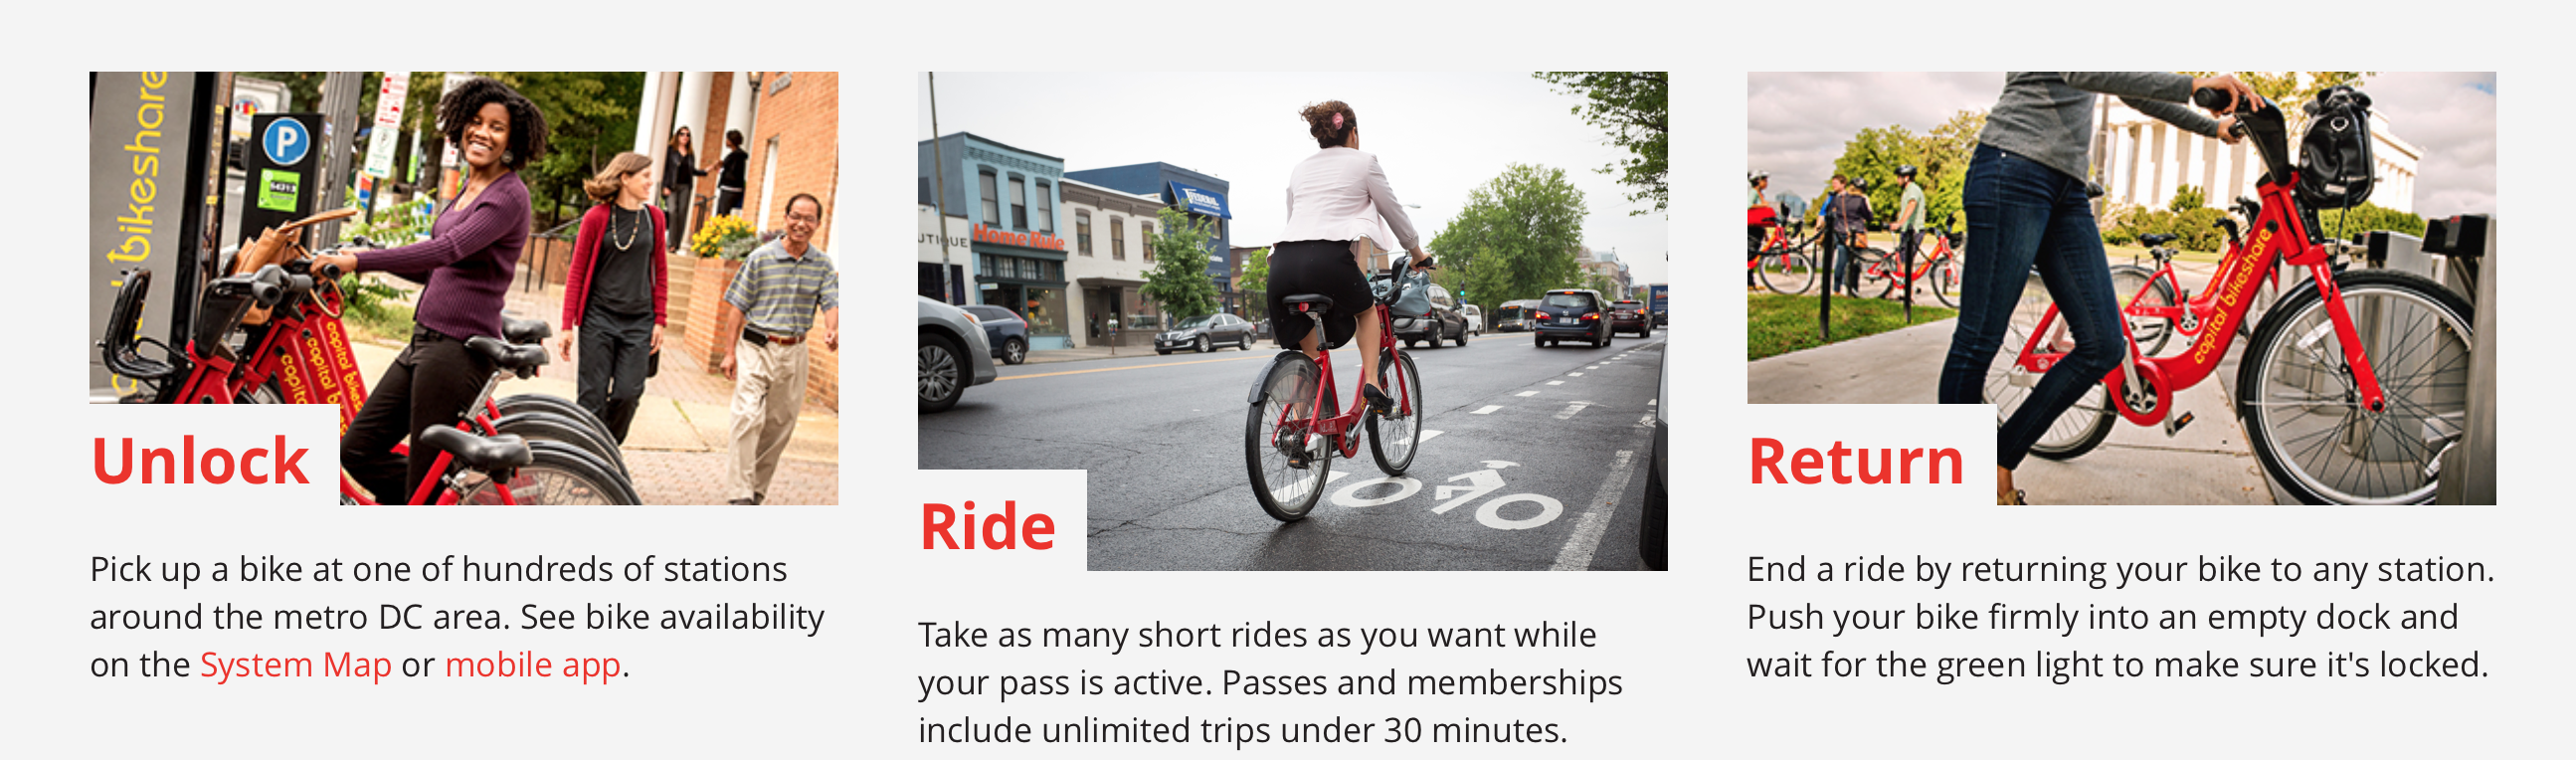
\includegraphics{fig/BSS.png}
\caption{bike\_sharing}
\end{figure}

Main Theme: Multiple Linear Regression, Subset Selection, Polynomial
Regression

\subsubsection{Overview}\label{overview}

You are hired by the administrators of the
\href{https://www.capitalbikeshare.com}{Capital Bikeshare program}
program in Washington D.C., to \textbf{help them predict the hourly
demand for rental bikes} and \textbf{give them suggestions on how to
increase their revenue}. Your task is to prepare a short report
summarizing your findings and make recommendations.

The predicted hourly demand could be used for planning the number of
bikes that need to be available in the system at any given hour of the
day. It costs the program money if bike stations are full and bikes
cannot be returned, or empty and there are no bikes available. You will
use multiple linear regression and polynomial regression and will
explore techniques for subset selection to predict bike usage. The goal
is to build a regression model that can predict the total number of bike
rentals in a given hour of the day, based on all available information
given to you.

An example of a suggestion to increase revenue might be to offer
discounts during certain times of the day either during holidays or
non-holidays. Your suggestions will depend on your observations of the
seasonality of ridership.

The data for this problem were collected from the Capital Bikeshare
program over the course of two years (2011 and 2012).

    \subsubsection{Use only the libraries
below:}\label{use-only-the-libraries-below}

    \begin{Verbatim}[commandchars=\\\{\}]
{\color{incolor}In [{\color{incolor}2}]:} \PY{k+kn}{import} \PY{n+nn}{numpy} \PY{k}{as} \PY{n+nn}{np}
        \PY{k+kn}{import} \PY{n+nn}{pandas} \PY{k}{as} \PY{n+nn}{pd}
        \PY{k+kn}{import} \PY{n+nn}{matplotlib}
        \PY{k+kn}{import} \PY{n+nn}{matplotlib}\PY{n+nn}{.}\PY{n+nn}{pyplot} \PY{k}{as} \PY{n+nn}{plt}
        
        \PY{k+kn}{import} \PY{n+nn}{statsmodels}\PY{n+nn}{.}\PY{n+nn}{api} \PY{k}{as} \PY{n+nn}{sm}
        \PY{k+kn}{from} \PY{n+nn}{statsmodels}\PY{n+nn}{.}\PY{n+nn}{api} \PY{k}{import} \PY{n}{OLS}
        
        \PY{k+kn}{from} \PY{n+nn}{sklearn} \PY{k}{import} \PY{n}{preprocessing}
        \PY{k+kn}{from} \PY{n+nn}{sklearn}\PY{n+nn}{.}\PY{n+nn}{preprocessing} \PY{k}{import} \PY{n}{PolynomialFeatures}
        \PY{k+kn}{from} \PY{n+nn}{sklearn}\PY{n+nn}{.}\PY{n+nn}{metrics} \PY{k}{import} \PY{n}{r2\PYZus{}score}
        \PY{k+kn}{from} \PY{n+nn}{sklearn}\PY{n+nn}{.}\PY{n+nn}{model\PYZus{}selection} \PY{k}{import} \PY{n}{train\PYZus{}test\PYZus{}split}
        
        \PY{k+kn}{from} \PY{n+nn}{pandas}\PY{n+nn}{.}\PY{n+nn}{plotting} \PY{k}{import} \PY{n}{scatter\PYZus{}matrix}
        
        \PY{k+kn}{import} \PY{n+nn}{seaborn} \PY{k}{as} \PY{n+nn}{sns}
        
        
        \PY{o}{\PYZpc{}}\PY{k}{matplotlib} inline
\end{Verbatim}


    \begin{Verbatim}[commandchars=\\\{\}]
{\color{incolor}In [{\color{incolor}3}]:} \PY{n}{plt}\PY{o}{.}\PY{n}{style}\PY{o}{.}\PY{n}{use}\PY{p}{(}\PY{l+s+s1}{\PYZsq{}}\PY{l+s+s1}{seaborn}\PY{l+s+s1}{\PYZsq{}}\PY{p}{)}
\end{Verbatim}


    \subsection{Data Exploration \& Preprocessing, Multiple Linear
Regression, Subset
Selection}\label{data-exploration-preprocessing-multiple-linear-regression-subset-selection}

    \subsubsection{Overview}\label{overview}

The initial data set is provided in the file
\texttt{data/BSS\_hour\_raw.csv}. You will first add features that will
help with the analysis and then separate the data into training and test
sets. Each row in this file represents the number of rides by registered
users and casual users in a given hour of a specific date. There are 12
attributes in total describing besides the number of users the weather
if it is a holiday or not etc:

\begin{itemize}
\tightlist
\item
  \texttt{dteday} (date in the format YYYY-MM-DD, e.g. 2011-01-01)
\item
  \texttt{season} (1 = winter, 2 = spring, 3 = summer, 4 = fall)
\item
  \texttt{hour} (0 for 12 midnight, 1 for 1:00am, 23 for 11:00pm)
\item
  \texttt{weekday} (0 through 6, with 0 denoting Sunday)
\item
  \texttt{holiday} (1 = the day is a holiday, 0 = otherwise)
\item
  \texttt{weather}

  \begin{itemize}
  \tightlist
  \item
    1: Clear, Few clouds, Partly cloudy, Partly cloudy
  \item
    2: Mist + Cloudy, Mist + Broken clouds, Mist + Few clouds, Mist
  \item
    3: Light Snow, Light Rain + Thunderstorm
  \item
    4: Heavy Rain + Thunderstorm + Mist, Snow + Fog
  \end{itemize}
\item
  \texttt{temp} (temperature in Celsius)
\item
  \texttt{atemp} (apparent temperature, or relative outdoor temperature,
  in Celsius)
\item
  \texttt{hum} (relative humidity)
\item
  \texttt{windspeed} (wind speed)
\item
  \texttt{casual} (number of rides that day made by casual riders, not
  registered in the system)
\item
  \texttt{registered} (number of rides that day made by registered
  riders)
\end{itemize}

    \subsubsection{General Hints}\label{general-hints}

\begin{itemize}
\tightlist
\item
  Use pandas .describe() to see statistics for the dataset.
\item
  When performing manipulations on column data it is useful and often
  more efficient to write a function and apply this function to the
  column as a whole without the need for iterating through the elements.
\item
  A scatterplot matrix or correlation matrix are both good ways to see
  dependencies between multiple variables.
\item
  For Question 2, a very useful pandas method is .groupby(). Make sure
  you aggregate the rest of the columns in a meaningful way. Print the
  dataframe to make sure all variables/columns are there!
\end{itemize}

\subsubsection{Resources}\label{resources}

http://pandas.pydata.org/pandas-docs/stable/generated/pandas.to\_datetime.html

     Question 1: Data Read-In and Cleaning

In this section, we read in the data and begin one of the most important
analytic steps: verifying that the data is what it claims to be.

\textbf{1.1} Load the dataset from the csv file
\texttt{data/BSS\_hour\_raw.csv} into a pandas dataframe that you name
\texttt{bikes\_df}. Do any of the variables' ranges or averages seem
suspect? Do the data types make sense?

\textbf{1.2} Notice that the variable in column \texttt{dteday} is a
pandas \texttt{object}, which is \textbf{not} useful when you want to
extract the elements of the date such as the year, month, and day.
Convert \texttt{dteday} into a \texttt{datetime} object to prepare it
for later analysis.

\textbf{1.3} Create three new columns in the dataframe: - \texttt{year}
with 0 for 2011, 1 for 2012, etc. - \texttt{month} with 1 through 12,
with 1 denoting January. - \texttt{counts} with the total number of bike
rentals for that \textbf{hour} (this is the response variable for
later).

    \subsubsection{Answers}\label{answers}

    \paragraph{\texorpdfstring{\textbf{1.1} Load the dataset from the csv
file \texttt{data/BSS\_hour\_raw.csv} into a pandas dataframe that you
name \texttt{bikes\_df}. Do any of the variables' ranges or averages
seem suspect? Do the data types make
sense?}{1.1 Load the dataset from the csv file data/BSS\_hour\_raw.csv into a pandas dataframe that you name bikes\_df. Do any of the variables' ranges or averages seem suspect? Do the data types make sense?}}\label{load-the-dataset-from-the-csv-file-databss_hour_raw.csv-into-a-pandas-dataframe-that-you-name-bikes_df.-do-any-of-the-variables-ranges-or-averages-seem-suspect-do-the-data-types-make-sense}

    \begin{Verbatim}[commandchars=\\\{\}]
{\color{incolor}In [{\color{incolor}4}]:} \PY{c+c1}{\PYZsh{} your code here}
        \PY{n}{df} \PY{o}{=} \PY{n}{pd}\PY{o}{.}\PY{n}{read\PYZus{}csv}\PY{p}{(}\PY{l+s+s1}{\PYZsq{}}\PY{l+s+s1}{./data/BSS\PYZus{}hour\PYZus{}raw.csv}\PY{l+s+s1}{\PYZsq{}}\PY{p}{)}
        \PY{n}{df}\PY{o}{.}\PY{n}{head}\PY{p}{(}\PY{p}{)}
\end{Verbatim}


\begin{Verbatim}[commandchars=\\\{\}]
{\color{outcolor}Out[{\color{outcolor}4}]:}        dteday  season  hour  holiday  weekday  workingday  weather  temp  \textbackslash{}
        0  2011-01-01       1     0        0        6           0        1  0.24   
        1  2011-01-01       1     1        0        6           0        1  0.22   
        2  2011-01-01       1     2        0        6           0        1  0.22   
        3  2011-01-01       1     3        0        6           0        1  0.24   
        4  2011-01-01       1     4        0        6           0        1  0.24   
        
            atemp   hum  windspeed  casual  registered  
        0  0.2879  0.81        0.0       3          13  
        1  0.2727  0.80        0.0       8          32  
        2  0.2727  0.80        0.0       5          27  
        3  0.2879  0.75        0.0       3          10  
        4  0.2879  0.75        0.0       0           1  
\end{Verbatim}
            
    \begin{Verbatim}[commandchars=\\\{\}]
{\color{incolor}In [{\color{incolor}5}]:} \PY{c+c1}{\PYZsh{} your code here}
        \PY{n}{df}\PY{o}{.}\PY{n}{describe}\PY{p}{(}\PY{p}{)}
\end{Verbatim}


\begin{Verbatim}[commandchars=\\\{\}]
{\color{outcolor}Out[{\color{outcolor}5}]:}              season          hour       holiday       weekday    workingday  \textbackslash{}
        count  17379.000000  17379.000000  17379.000000  17379.000000  17379.000000   
        mean       2.501640     11.546752      0.028770      3.003683      0.682721   
        std        1.106918      6.914405      0.167165      2.005771      0.465431   
        min        1.000000      0.000000      0.000000      0.000000      0.000000   
        25\%        2.000000      6.000000      0.000000      1.000000      0.000000   
        50\%        3.000000     12.000000      0.000000      3.000000      1.000000   
        75\%        3.000000     18.000000      0.000000      5.000000      1.000000   
        max        4.000000     23.000000      1.000000      6.000000      1.000000   
        
                    weather          temp         atemp           hum     windspeed  \textbackslash{}
        count  17379.000000  17379.000000  17379.000000  17379.000000  17379.000000   
        mean       1.425283      0.496987      0.475775      0.627229      0.190098   
        std        0.639357      0.192556      0.171850      0.192930      0.122340   
        min        1.000000      0.020000      0.000000      0.000000      0.000000   
        25\%        1.000000      0.340000      0.333300      0.480000      0.104500   
        50\%        1.000000      0.500000      0.484800      0.630000      0.194000   
        75\%        2.000000      0.660000      0.621200      0.780000      0.253700   
        max        4.000000      1.000000      1.000000      1.000000      0.850700   
        
                     casual    registered  
        count  17379.000000  17379.000000  
        mean      35.676218    153.786869  
        std       49.305030    151.357286  
        min        0.000000      0.000000  
        25\%        4.000000     34.000000  
        50\%       17.000000    115.000000  
        75\%       48.000000    220.000000  
        max      367.000000    886.000000  
\end{Verbatim}
            
    \begin{Verbatim}[commandchars=\\\{\}]
{\color{incolor}In [{\color{incolor}6}]:} \PY{c+c1}{\PYZsh{} your code here}
        \PY{n}{df}\PY{o}{.}\PY{n}{dtypes}
\end{Verbatim}


\begin{Verbatim}[commandchars=\\\{\}]
{\color{outcolor}Out[{\color{outcolor}6}]:} dteday         object
        season          int64
        hour            int64
        holiday         int64
        weekday         int64
        workingday      int64
        weather         int64
        temp          float64
        atemp         float64
        hum           float64
        windspeed     float64
        casual          int64
        registered      int64
        dtype: object
\end{Verbatim}
            
    \emph{Your answer here}

Observations: * It is strange that \texttt{temp} and \texttt{atemp} have
maximums of 1 and are never negative. I am going to assume that these
values have been standardized to this range. * It is unclear what units
\texttt{windspeed} is measured in. * \texttt{dteday} should have a type
that represents that it is a date, not just a general "object"

    \paragraph{\texorpdfstring{\textbf{1.2} Notice that the variable in
column \texttt{dteday} is a pandas \texttt{object}, which is
\textbf{not} useful when you want to extract the elements of the date
such as the year, month, and day. Convert \texttt{dteday} into a
\texttt{datetime} object to prepare it for later
analysis.}{1.2 Notice that the variable in column dteday is a pandas object, which is not useful when you want to extract the elements of the date such as the year, month, and day. Convert dteday into a datetime object to prepare it for later analysis.}}\label{notice-that-the-variable-in-column-dteday-is-a-pandas-object-which-is-not-useful-when-you-want-to-extract-the-elements-of-the-date-such-as-the-year-month-and-day.-convert-dteday-into-a-datetime-object-to-prepare-it-for-later-analysis.}

    \begin{Verbatim}[commandchars=\\\{\}]
{\color{incolor}In [{\color{incolor}7}]:} \PY{c+c1}{\PYZsh{} your code here}
        \PY{n}{df}\PY{p}{[}\PY{l+s+s1}{\PYZsq{}}\PY{l+s+s1}{dteday}\PY{l+s+s1}{\PYZsq{}}\PY{p}{]} \PY{o}{=} \PY{n}{pd}\PY{o}{.}\PY{n}{to\PYZus{}datetime}\PY{p}{(}\PY{n}{df}\PY{p}{[}\PY{l+s+s1}{\PYZsq{}}\PY{l+s+s1}{dteday}\PY{l+s+s1}{\PYZsq{}}\PY{p}{]}\PY{p}{,} \PY{n+nb}{format}\PY{o}{=}\PY{l+s+s1}{\PYZsq{}}\PY{l+s+s1}{\PYZpc{}}\PY{l+s+s1}{Y\PYZhy{}}\PY{l+s+s1}{\PYZpc{}}\PY{l+s+s1}{m\PYZhy{}}\PY{l+s+si}{\PYZpc{}d}\PY{l+s+s1}{\PYZsq{}}\PY{p}{)}
        \PY{n}{df}\PY{o}{.}\PY{n}{dtypes}
\end{Verbatim}


\begin{Verbatim}[commandchars=\\\{\}]
{\color{outcolor}Out[{\color{outcolor}7}]:} dteday        datetime64[ns]
        season                 int64
        hour                   int64
        holiday                int64
        weekday                int64
        workingday             int64
        weather                int64
        temp                 float64
        atemp                float64
        hum                  float64
        windspeed            float64
        casual                 int64
        registered             int64
        dtype: object
\end{Verbatim}
            
    \paragraph{\texorpdfstring{\textbf{1.3} Create three new columns in the
dataframe:}{1.3 Create three new columns in the dataframe:}}\label{create-three-new-columns-in-the-dataframe}

\begin{itemize}
\tightlist
\item
  \texttt{year} with 0 for 2011, 1 for 2012, etc.
\item
  \texttt{month} with 1 through 12, with 1 denoting January.
\item
  \texttt{counts} with the total number of bike rentals for that hour
  (this is the response variable for later).
\end{itemize}

    \begin{Verbatim}[commandchars=\\\{\}]
{\color{incolor}In [{\color{incolor}8}]:} \PY{c+c1}{\PYZsh{} your code here}
        \PY{n}{df}\PY{p}{[}\PY{l+s+s1}{\PYZsq{}}\PY{l+s+s1}{year}\PY{l+s+s1}{\PYZsq{}}\PY{p}{]} \PY{o}{=} \PY{n}{df}\PY{p}{[}\PY{l+s+s1}{\PYZsq{}}\PY{l+s+s1}{dteday}\PY{l+s+s1}{\PYZsq{}}\PY{p}{]}\PY{o}{.}\PY{n}{apply}\PY{p}{(}\PY{k}{lambda} \PY{n}{x} \PY{p}{:} \PY{n}{x}\PY{o}{.}\PY{n}{year}\PY{p}{)}
        \PY{n}{df}\PY{p}{[}\PY{l+s+s1}{\PYZsq{}}\PY{l+s+s1}{month}\PY{l+s+s1}{\PYZsq{}}\PY{p}{]} \PY{o}{=} \PY{n}{df}\PY{p}{[}\PY{l+s+s1}{\PYZsq{}}\PY{l+s+s1}{dteday}\PY{l+s+s1}{\PYZsq{}}\PY{p}{]}\PY{o}{.}\PY{n}{apply}\PY{p}{(}\PY{k}{lambda} \PY{n}{x} \PY{p}{:} \PY{n}{x}\PY{o}{.}\PY{n}{month}\PY{p}{)}
        \PY{n}{df}\PY{p}{[}\PY{l+s+s1}{\PYZsq{}}\PY{l+s+s1}{counts}\PY{l+s+s1}{\PYZsq{}}\PY{p}{]}\PY{o}{=}\PY{n}{df}\PY{o}{.}\PY{n}{casual}\PY{o}{+}\PY{n}{df}\PY{o}{.}\PY{n}{registered}
\end{Verbatim}


    \begin{Verbatim}[commandchars=\\\{\}]
{\color{incolor}In [{\color{incolor}9}]:} \PY{c+c1}{\PYZsh{} your code here}
        \PY{n}{df}\PY{o}{.}\PY{n}{head}\PY{p}{(}\PY{p}{)}
\end{Verbatim}


\begin{Verbatim}[commandchars=\\\{\}]
{\color{outcolor}Out[{\color{outcolor}9}]:}       dteday  season  hour  holiday  weekday  workingday  weather  temp  \textbackslash{}
        0 2011-01-01       1     0        0        6           0        1  0.24   
        1 2011-01-01       1     1        0        6           0        1  0.22   
        2 2011-01-01       1     2        0        6           0        1  0.22   
        3 2011-01-01       1     3        0        6           0        1  0.24   
        4 2011-01-01       1     4        0        6           0        1  0.24   
        
            atemp   hum  windspeed  casual  registered  year  month  counts  
        0  0.2879  0.81        0.0       3          13  2011      1      16  
        1  0.2727  0.80        0.0       8          32  2011      1      40  
        2  0.2727  0.80        0.0       5          27  2011      1      32  
        3  0.2879  0.75        0.0       3          10  2011      1      13  
        4  0.2879  0.75        0.0       0           1  2011      1       1  
\end{Verbatim}
            
     Question 2: Exploratory Data Analysis.

In this question, we continue validating the data, and begin hunting for
patterns in ridership that shed light on who uses the service and why.

\textbf{2.1} Use pandas' \texttt{scatter\_matrix} command to visualize
the inter-dependencies among all predictors in the dataset. Note and
comment on any strongly related variables. {[}This will take several
minutes to run. You may wish to comment it out until your final
submission, or only plot a randomly-selected 10\% of the rows{]}

\textbf{2.2} Make a plot showing the \emph{average} number of casual and
registered riders during each hour of the day. \texttt{.groupby} and
\texttt{.aggregate} should make this task easy. Comment on the trends
you observe.

\textbf{2.3} Use the variable \texttt{weather} to show how each weather
category affects the relationships in question 2.2. What do you observe?

\textbf{2.4} Make a new dataframe with the following subset of
attributes from the previous dataset and with each entry being just
\textbf{one} day:

\begin{itemize}
\tightlist
\item
  \texttt{dteday}, the timestamp for that day (fine to set to noon or
  any other time)
\item
  \texttt{weekday}, the day of the week
\item
  \texttt{weather}, the most severe weather that day
\item
  \texttt{season}, the season that day falls in
\item
  \texttt{temp}, the average temperature (normalized)
\item
  \texttt{atemp}, the average atemp that day (normalized)
\item
  \texttt{windspeed}, the average windspeed that day (normalized)
\item
  \texttt{hum}, the average humidity that day (normalized)
\item
  \texttt{casual}, the \textbf{total} number of rentals by casual users
\item
  \texttt{registered}, the \textbf{total} number of rentals by
  registered users
\item
  \texttt{counts}, the \textbf{total} number of rentals of that day
\end{itemize}

Name this dataframe \texttt{bikes\_by\_day}.

Make a plot showing the \emph{distribution} of the number of casual and
registered riders on each day of the week.

\textbf{2.5} Use \texttt{bikes\_by\_day} to visualize how the
distribution of \textbf{total number of rides} per day (casual and
registered riders combined) varies with the \textbf{season}. Do you see
any \textbf{outliers}? Here we use the pyplot's boxplot function
definition of an outlier as any value 1.5 times the IQR above the 75th
percentile or 1.5 times the IQR below the 25th percentiles. If you see
any outliers, identify those dates and investigate if they are a chance
occurence, an error in the data collection, or a significant event (an
online search of those date(s) might help).

    \subsubsection{Answers}\label{answers}

    \paragraph{\texorpdfstring{\textbf{2.1} Use pandas'
\texttt{scatter\_matrix} command to visualize the inter-dependencies
among all predictors in the dataset. Note and comment on any strongly
related variables. {[}This will take several minutes to run. You may
wish to comment it out until your final submission, or only plot a
randomly-selected 10\% of the
rows{]}}{2.1 Use pandas' scatter\_matrix command to visualize the inter-dependencies among all predictors in the dataset. Note and comment on any strongly related variables. {[}This will take several minutes to run. You may wish to comment it out until your final submission, or only plot a randomly-selected 10\% of the rows{]}}}\label{use-pandas-scatter_matrix-command-to-visualize-the-inter-dependencies-among-all-predictors-in-the-dataset.-note-and-comment-on-any-strongly-related-variables.-this-will-take-several-minutes-to-run.-you-may-wish-to-comment-it-out-until-your-final-submission-or-only-plot-a-randomly-selected-10-of-the-rows}

    \begin{Verbatim}[commandchars=\\\{\}]
{\color{incolor}In [{\color{incolor}10}]:} \PY{c+c1}{\PYZsh{} your code here}
         \PY{n}{plot} \PY{o}{=} \PY{n}{pd}\PY{o}{.}\PY{n}{scatter\PYZus{}matrix}\PY{p}{(}\PY{n}{df}\PY{p}{,} \PY{n}{figsize} \PY{o}{=} \PY{p}{(}\PY{l+m+mi}{14}\PY{p}{,} \PY{l+m+mi}{14}\PY{p}{)}\PY{p}{)}
         \PY{n}{plot}
\end{Verbatim}


    \begin{Verbatim}[commandchars=\\\{\}]
/Users/joshfeldman/anaconda3/envs/py36/lib/python3.6/site-packages/ipykernel/\_\_main\_\_.py:2: FutureWarning: pandas.scatter\_matrix is deprecated, use pandas.plotting.scatter\_matrix instead
  from ipykernel import kernelapp as app

    \end{Verbatim}

\begin{Verbatim}[commandchars=\\\{\}]
{\color{outcolor}Out[{\color{outcolor}10}]:} array([[<matplotlib.axes.\_subplots.AxesSubplot object at 0x10c5bb9b0>,
                 <matplotlib.axes.\_subplots.AxesSubplot object at 0x11ca61f28>,
                 <matplotlib.axes.\_subplots.AxesSubplot object at 0x11ca8f9e8>,
                 <matplotlib.axes.\_subplots.AxesSubplot object at 0x11cac14a8>,
                 <matplotlib.axes.\_subplots.AxesSubplot object at 0x11cae6f28>,
                 <matplotlib.axes.\_subplots.AxesSubplot object at 0x11cae6f60>,
                 <matplotlib.axes.\_subplots.AxesSubplot object at 0x11cb414a8>,
                 <matplotlib.axes.\_subplots.AxesSubplot object at 0x11cb66f28>,
                 <matplotlib.axes.\_subplots.AxesSubplot object at 0x11cb939e8>,
                 <matplotlib.axes.\_subplots.AxesSubplot object at 0x11cbc64a8>,
                 <matplotlib.axes.\_subplots.AxesSubplot object at 0x11cbecf28>,
                 <matplotlib.axes.\_subplots.AxesSubplot object at 0x11cc9c9e8>,
                 <matplotlib.axes.\_subplots.AxesSubplot object at 0x11ccc94a8>,
                 <matplotlib.axes.\_subplots.AxesSubplot object at 0x11ca2bf28>,
                 <matplotlib.axes.\_subplots.AxesSubplot object at 0x11cc1a9e8>],
                [<matplotlib.axes.\_subplots.AxesSubplot object at 0x11cc474a8>,
                 <matplotlib.axes.\_subplots.AxesSubplot object at 0x10c5e1f28>,
                 <matplotlib.axes.\_subplots.AxesSubplot object at 0x11224c9e8>,
                 <matplotlib.axes.\_subplots.AxesSubplot object at 0x11227a4a8>,
                 <matplotlib.axes.\_subplots.AxesSubplot object at 0x11cc76f28>,
                 <matplotlib.axes.\_subplots.AxesSubplot object at 0x11cce39e8>,
                 <matplotlib.axes.\_subplots.AxesSubplot object at 0x11cd124a8>,
                 <matplotlib.axes.\_subplots.AxesSubplot object at 0x11cd36f28>,
                 <matplotlib.axes.\_subplots.AxesSubplot object at 0x11cd659e8>,
                 <matplotlib.axes.\_subplots.AxesSubplot object at 0x11cd954a8>,
                 <matplotlib.axes.\_subplots.AxesSubplot object at 0x11cdb9ef0>,
                 <matplotlib.axes.\_subplots.AxesSubplot object at 0x11db519b0>,
                 <matplotlib.axes.\_subplots.AxesSubplot object at 0x1c21366470>,
                 <matplotlib.axes.\_subplots.AxesSubplot object at 0x1c2138cef0>,
                 <matplotlib.axes.\_subplots.AxesSubplot object at 0x1c213b99b0>],
                [<matplotlib.axes.\_subplots.AxesSubplot object at 0x1c213e8470>,
                 <matplotlib.axes.\_subplots.AxesSubplot object at 0x1c2140def0>,
                 <matplotlib.axes.\_subplots.AxesSubplot object at 0x1c214399b0>,
                 <matplotlib.axes.\_subplots.AxesSubplot object at 0x1c2146a470>,
                 <matplotlib.axes.\_subplots.AxesSubplot object at 0x1c21490ef0>,
                 <matplotlib.axes.\_subplots.AxesSubplot object at 0x1c214be9b0>,
                 <matplotlib.axes.\_subplots.AxesSubplot object at 0x1c214ed470>,
                 <matplotlib.axes.\_subplots.AxesSubplot object at 0x1c21512ef0>,
                 <matplotlib.axes.\_subplots.AxesSubplot object at 0x1c2153f9b0>,
                 <matplotlib.axes.\_subplots.AxesSubplot object at 0x1c2156f470>,
                 <matplotlib.axes.\_subplots.AxesSubplot object at 0x1c21593ef0>,
                 <matplotlib.axes.\_subplots.AxesSubplot object at 0x1c215c09b0>,
                 <matplotlib.axes.\_subplots.AxesSubplot object at 0x1c215f2470>,
                 <matplotlib.axes.\_subplots.AxesSubplot object at 0x1c21617ef0>,
                 <matplotlib.axes.\_subplots.AxesSubplot object at 0x1c216469b0>],
                [<matplotlib.axes.\_subplots.AxesSubplot object at 0x1c21675470>,
                 <matplotlib.axes.\_subplots.AxesSubplot object at 0x1c21698ef0>,
                 <matplotlib.axes.\_subplots.AxesSubplot object at 0x1c216c69b0>,
                 <matplotlib.axes.\_subplots.AxesSubplot object at 0x1c216f5470>,
                 <matplotlib.axes.\_subplots.AxesSubplot object at 0x1c2171bef0>,
                 <matplotlib.axes.\_subplots.AxesSubplot object at 0x1c2174a9b0>,
                 <matplotlib.axes.\_subplots.AxesSubplot object at 0x1c21779470>,
                 <matplotlib.axes.\_subplots.AxesSubplot object at 0x1c2179fef0>,
                 <matplotlib.axes.\_subplots.AxesSubplot object at 0x1c217cc9b0>,
                 <matplotlib.axes.\_subplots.AxesSubplot object at 0x1c217fa470>,
                 <matplotlib.axes.\_subplots.AxesSubplot object at 0x1c21820ef0>,
                 <matplotlib.axes.\_subplots.AxesSubplot object at 0x1c2184e9b0>,
                 <matplotlib.axes.\_subplots.AxesSubplot object at 0x1c2187d470>,
                 <matplotlib.axes.\_subplots.AxesSubplot object at 0x1c2253bef0>,
                 <matplotlib.axes.\_subplots.AxesSubplot object at 0x1c225699b0>],
                [<matplotlib.axes.\_subplots.AxesSubplot object at 0x1c22595470>,
                 <matplotlib.axes.\_subplots.AxesSubplot object at 0x1c225beef0>,
                 <matplotlib.axes.\_subplots.AxesSubplot object at 0x1c225e99b0>,
                 <matplotlib.axes.\_subplots.AxesSubplot object at 0x1c2261b470>,
                 <matplotlib.axes.\_subplots.AxesSubplot object at 0x1c22640ef0>,
                 <matplotlib.axes.\_subplots.AxesSubplot object at 0x1c2266b9b0>,
                 <matplotlib.axes.\_subplots.AxesSubplot object at 0x1c2269d470>,
                 <matplotlib.axes.\_subplots.AxesSubplot object at 0x1c226c3ef0>,
                 <matplotlib.axes.\_subplots.AxesSubplot object at 0x1c226f19b0>,
                 <matplotlib.axes.\_subplots.AxesSubplot object at 0x1c2271f470>,
                 <matplotlib.axes.\_subplots.AxesSubplot object at 0x1c22745ef0>,
                 <matplotlib.axes.\_subplots.AxesSubplot object at 0x1c227719b0>,
                 <matplotlib.axes.\_subplots.AxesSubplot object at 0x1c2279f400>,
                 <matplotlib.axes.\_subplots.AxesSubplot object at 0x1c227c6e80>,
                 <matplotlib.axes.\_subplots.AxesSubplot object at 0x1c227f4940>],
                [<matplotlib.axes.\_subplots.AxesSubplot object at 0x1c22825400>,
                 <matplotlib.axes.\_subplots.AxesSubplot object at 0x1c2284ae80>,
                 <matplotlib.axes.\_subplots.AxesSubplot object at 0x1c22879940>,
                 <matplotlib.axes.\_subplots.AxesSubplot object at 0x1c228a6400>,
                 <matplotlib.axes.\_subplots.AxesSubplot object at 0x1c228cae80>,
                 <matplotlib.axes.\_subplots.AxesSubplot object at 0x1c228f9940>,
                 <matplotlib.axes.\_subplots.AxesSubplot object at 0x1c22929400>,
                 <matplotlib.axes.\_subplots.AxesSubplot object at 0x1c2294ee80>,
                 <matplotlib.axes.\_subplots.AxesSubplot object at 0x1c2297d940>,
                 <matplotlib.axes.\_subplots.AxesSubplot object at 0x1c229a9400>,
                 <matplotlib.axes.\_subplots.AxesSubplot object at 0x1c229d0e80>,
                 <matplotlib.axes.\_subplots.AxesSubplot object at 0x1c229ff940>,
                 <matplotlib.axes.\_subplots.AxesSubplot object at 0x1c22a2c400>,
                 <matplotlib.axes.\_subplots.AxesSubplot object at 0x1c22a53e80>,
                 <matplotlib.axes.\_subplots.AxesSubplot object at 0x1c22a81940>],
                [<matplotlib.axes.\_subplots.AxesSubplot object at 0x1c22ab2400>,
                 <matplotlib.axes.\_subplots.AxesSubplot object at 0x1c22ad7e80>,
                 <matplotlib.axes.\_subplots.AxesSubplot object at 0x1c22b05940>,
                 <matplotlib.axes.\_subplots.AxesSubplot object at 0x1c22b32400>,
                 <matplotlib.axes.\_subplots.AxesSubplot object at 0x1c22b59e80>,
                 <matplotlib.axes.\_subplots.AxesSubplot object at 0x1c22b86940>,
                 <matplotlib.axes.\_subplots.AxesSubplot object at 0x1c22bb6400>,
                 <matplotlib.axes.\_subplots.AxesSubplot object at 0x1c22bdae80>,
                 <matplotlib.axes.\_subplots.AxesSubplot object at 0x1c22c09940>,
                 <matplotlib.axes.\_subplots.AxesSubplot object at 0x1c22c3a400>,
                 <matplotlib.axes.\_subplots.AxesSubplot object at 0x1c22c5ee80>,
                 <matplotlib.axes.\_subplots.AxesSubplot object at 0x1c22c8b940>,
                 <matplotlib.axes.\_subplots.AxesSubplot object at 0x1c22cb9400>,
                 <matplotlib.axes.\_subplots.AxesSubplot object at 0x1c22ce0e80>,
                 <matplotlib.axes.\_subplots.AxesSubplot object at 0x1c22d0d940>],
                [<matplotlib.axes.\_subplots.AxesSubplot object at 0x1c22d3c400>,
                 <matplotlib.axes.\_subplots.AxesSubplot object at 0x1c22d61e80>,
                 <matplotlib.axes.\_subplots.AxesSubplot object at 0x1c22d90940>,
                 <matplotlib.axes.\_subplots.AxesSubplot object at 0x1c22dbf400>,
                 <matplotlib.axes.\_subplots.AxesSubplot object at 0x1c22de5e80>,
                 <matplotlib.axes.\_subplots.AxesSubplot object at 0x1c22e13940>,
                 <matplotlib.axes.\_subplots.AxesSubplot object at 0x1c22e40400>,
                 <matplotlib.axes.\_subplots.AxesSubplot object at 0x1c22e65e80>,
                 <matplotlib.axes.\_subplots.AxesSubplot object at 0x1c22e95940>,
                 <matplotlib.axes.\_subplots.AxesSubplot object at 0x1c22ec7400>,
                 <matplotlib.axes.\_subplots.AxesSubplot object at 0x1c22eeae80>,
                 <matplotlib.axes.\_subplots.AxesSubplot object at 0x1c22f18940>,
                 <matplotlib.axes.\_subplots.AxesSubplot object at 0x1c22f46400>,
                 <matplotlib.axes.\_subplots.AxesSubplot object at 0x1c22f6ce80>,
                 <matplotlib.axes.\_subplots.AxesSubplot object at 0x1c22f97940>],
                [<matplotlib.axes.\_subplots.AxesSubplot object at 0x1c22fc8400>,
                 <matplotlib.axes.\_subplots.AxesSubplot object at 0x1c22fefe80>,
                 <matplotlib.axes.\_subplots.AxesSubplot object at 0x1c2301c940>,
                 <matplotlib.axes.\_subplots.AxesSubplot object at 0x1c2304c400>,
                 <matplotlib.axes.\_subplots.AxesSubplot object at 0x1c23071e80>,
                 <matplotlib.axes.\_subplots.AxesSubplot object at 0x1c2309f940>,
                 <matplotlib.axes.\_subplots.AxesSubplot object at 0x1c230cd400>,
                 <matplotlib.axes.\_subplots.AxesSubplot object at 0x1c230f3e80>,
                 <matplotlib.axes.\_subplots.AxesSubplot object at 0x1c23121940>,
                 <matplotlib.axes.\_subplots.AxesSubplot object at 0x1c2314f400>,
                 <matplotlib.axes.\_subplots.AxesSubplot object at 0x1c23175e80>,
                 <matplotlib.axes.\_subplots.AxesSubplot object at 0x1c231a3940>,
                 <matplotlib.axes.\_subplots.AxesSubplot object at 0x1c231d2400>,
                 <matplotlib.axes.\_subplots.AxesSubplot object at 0x1c231f7e80>,
                 <matplotlib.axes.\_subplots.AxesSubplot object at 0x1c23226940>],
                [<matplotlib.axes.\_subplots.AxesSubplot object at 0x1c23254400>,
                 <matplotlib.axes.\_subplots.AxesSubplot object at 0x1c2327ae80>,
                 <matplotlib.axes.\_subplots.AxesSubplot object at 0x1c232a7940>,
                 <matplotlib.axes.\_subplots.AxesSubplot object at 0x1c232d8400>,
                 <matplotlib.axes.\_subplots.AxesSubplot object at 0x1c232fee80>,
                 <matplotlib.axes.\_subplots.AxesSubplot object at 0x1c2332c940>,
                 <matplotlib.axes.\_subplots.AxesSubplot object at 0x1c2335a400>,
                 <matplotlib.axes.\_subplots.AxesSubplot object at 0x1c2337ee80>,
                 <matplotlib.axes.\_subplots.AxesSubplot object at 0x1c233ae940>,
                 <matplotlib.axes.\_subplots.AxesSubplot object at 0x1c233dc400>,
                 <matplotlib.axes.\_subplots.AxesSubplot object at 0x1c23400e80>,
                 <matplotlib.axes.\_subplots.AxesSubplot object at 0x1c2342f940>,
                 <matplotlib.axes.\_subplots.AxesSubplot object at 0x1c2345f400>,
                 <matplotlib.axes.\_subplots.AxesSubplot object at 0x1c23483e80>,
                 <matplotlib.axes.\_subplots.AxesSubplot object at 0x1c234b4940>],
                [<matplotlib.axes.\_subplots.AxesSubplot object at 0x1c234e1400>,
                 <matplotlib.axes.\_subplots.AxesSubplot object at 0x1c23505e80>,
                 <matplotlib.axes.\_subplots.AxesSubplot object at 0x1c23532940>,
                 <matplotlib.axes.\_subplots.AxesSubplot object at 0x1c23563400>,
                 <matplotlib.axes.\_subplots.AxesSubplot object at 0x1c23589e80>,
                 <matplotlib.axes.\_subplots.AxesSubplot object at 0x1c235b6940>,
                 <matplotlib.axes.\_subplots.AxesSubplot object at 0x1c235e4400>,
                 <matplotlib.axes.\_subplots.AxesSubplot object at 0x1c2360be80>,
                 <matplotlib.axes.\_subplots.AxesSubplot object at 0x1c23639940>,
                 <matplotlib.axes.\_subplots.AxesSubplot object at 0x1c23669400>,
                 <matplotlib.axes.\_subplots.AxesSubplot object at 0x1c2368fe80>,
                 <matplotlib.axes.\_subplots.AxesSubplot object at 0x1c236bb940>,
                 <matplotlib.axes.\_subplots.AxesSubplot object at 0x1c236ec400>,
                 <matplotlib.axes.\_subplots.AxesSubplot object at 0x1c23711e80>,
                 <matplotlib.axes.\_subplots.AxesSubplot object at 0x1c2373d940>],
                [<matplotlib.axes.\_subplots.AxesSubplot object at 0x1c2376c400>,
                 <matplotlib.axes.\_subplots.AxesSubplot object at 0x1c23792e80>,
                 <matplotlib.axes.\_subplots.AxesSubplot object at 0x1c237c1940>,
                 <matplotlib.axes.\_subplots.AxesSubplot object at 0x1c237f0400>,
                 <matplotlib.axes.\_subplots.AxesSubplot object at 0x1c23815e80>,
                 <matplotlib.axes.\_subplots.AxesSubplot object at 0x1c23843940>,
                 <matplotlib.axes.\_subplots.AxesSubplot object at 0x1c23873400>,
                 <matplotlib.axes.\_subplots.AxesSubplot object at 0x1c2389ae80>,
                 <matplotlib.axes.\_subplots.AxesSubplot object at 0x1c238c6940>,
                 <matplotlib.axes.\_subplots.AxesSubplot object at 0x1c238f4400>,
                 <matplotlib.axes.\_subplots.AxesSubplot object at 0x1c2391ae80>,
                 <matplotlib.axes.\_subplots.AxesSubplot object at 0x1c23948940>,
                 <matplotlib.axes.\_subplots.AxesSubplot object at 0x1c23976400>,
                 <matplotlib.axes.\_subplots.AxesSubplot object at 0x1c2399ee80>,
                 <matplotlib.axes.\_subplots.AxesSubplot object at 0x1c239cc940>],
                [<matplotlib.axes.\_subplots.AxesSubplot object at 0x1c239f9400>,
                 <matplotlib.axes.\_subplots.AxesSubplot object at 0x1c23a1de80>,
                 <matplotlib.axes.\_subplots.AxesSubplot object at 0x1c23a4f940>,
                 <matplotlib.axes.\_subplots.AxesSubplot object at 0x1c23a7b400>,
                 <matplotlib.axes.\_subplots.AxesSubplot object at 0x1c23aa2e80>,
                 <matplotlib.axes.\_subplots.AxesSubplot object at 0x1c23ad0940>,
                 <matplotlib.axes.\_subplots.AxesSubplot object at 0x1c23aff400>,
                 <matplotlib.axes.\_subplots.AxesSubplot object at 0x1c23b26e80>,
                 <matplotlib.axes.\_subplots.AxesSubplot object at 0x1c23b52940>,
                 <matplotlib.axes.\_subplots.AxesSubplot object at 0x1c23b82400>,
                 <matplotlib.axes.\_subplots.AxesSubplot object at 0x1c23ba6e80>,
                 <matplotlib.axes.\_subplots.AxesSubplot object at 0x1c23bd3940>,
                 <matplotlib.axes.\_subplots.AxesSubplot object at 0x1c23c04400>,
                 <matplotlib.axes.\_subplots.AxesSubplot object at 0x1c23c29e80>,
                 <matplotlib.axes.\_subplots.AxesSubplot object at 0x1c23c57940>],
                [<matplotlib.axes.\_subplots.AxesSubplot object at 0x1c23c86400>,
                 <matplotlib.axes.\_subplots.AxesSubplot object at 0x1c23cace80>,
                 <matplotlib.axes.\_subplots.AxesSubplot object at 0x1c23cd9940>,
                 <matplotlib.axes.\_subplots.AxesSubplot object at 0x1c23d09400>,
                 <matplotlib.axes.\_subplots.AxesSubplot object at 0x1c23d2de80>,
                 <matplotlib.axes.\_subplots.AxesSubplot object at 0x1c23d5a940>,
                 <matplotlib.axes.\_subplots.AxesSubplot object at 0x1c23d8a400>,
                 <matplotlib.axes.\_subplots.AxesSubplot object at 0x1c23db0e80>,
                 <matplotlib.axes.\_subplots.AxesSubplot object at 0x1c23ddf940>,
                 <matplotlib.axes.\_subplots.AxesSubplot object at 0x1c23e0d400>,
                 <matplotlib.axes.\_subplots.AxesSubplot object at 0x1c23e32e80>,
                 <matplotlib.axes.\_subplots.AxesSubplot object at 0x1c23e61940>,
                 <matplotlib.axes.\_subplots.AxesSubplot object at 0x1c23e91400>,
                 <matplotlib.axes.\_subplots.AxesSubplot object at 0x1c23eb6e80>,
                 <matplotlib.axes.\_subplots.AxesSubplot object at 0x1c23ee3940>],
                [<matplotlib.axes.\_subplots.AxesSubplot object at 0x1c23f11400>,
                 <matplotlib.axes.\_subplots.AxesSubplot object at 0x1c23f38e80>,
                 <matplotlib.axes.\_subplots.AxesSubplot object at 0x1c23f66940>,
                 <matplotlib.axes.\_subplots.AxesSubplot object at 0x1c23f95400>,
                 <matplotlib.axes.\_subplots.AxesSubplot object at 0x1c23fbae80>,
                 <matplotlib.axes.\_subplots.AxesSubplot object at 0x1c23fe7940>,
                 <matplotlib.axes.\_subplots.AxesSubplot object at 0x1c24015400>,
                 <matplotlib.axes.\_subplots.AxesSubplot object at 0x1c2403de80>,
                 <matplotlib.axes.\_subplots.AxesSubplot object at 0x1c2406a940>,
                 <matplotlib.axes.\_subplots.AxesSubplot object at 0x1c2409a400>,
                 <matplotlib.axes.\_subplots.AxesSubplot object at 0x1c240bde80>,
                 <matplotlib.axes.\_subplots.AxesSubplot object at 0x1c240ed940>,
                 <matplotlib.axes.\_subplots.AxesSubplot object at 0x1c2411c400>,
                 <matplotlib.axes.\_subplots.AxesSubplot object at 0x1c24140e80>,
                 <matplotlib.axes.\_subplots.AxesSubplot object at 0x1c2416e940>]],
               dtype=object)
\end{Verbatim}
            
    \begin{center}
    \adjustimage{max size={0.9\linewidth}{0.9\paperheight}}{output_26_2.png}
    \end{center}
    { \hspace*{\fill} \\}
    
    \emph{your answer here}

There are some collinearities in the data. Notably, temp vs. atemp vs.
month vs. season. There seems to be a lot of structure in the data
relating counts to various times (hour, holiday, weekday, workingday,
month).

    \paragraph{\texorpdfstring{\textbf{2.2} Make a plot showing the
\emph{average} number of casual and registered riders during each hour
of the day. \texttt{.groupby} and \texttt{.aggregate} should make this
task easy. Comment on the trends you
observe.}{2.2 Make a plot showing the average number of casual and registered riders during each hour of the day. .groupby and .aggregate should make this task easy. Comment on the trends you observe.}}\label{make-a-plot-showing-the-average-number-of-casual-and-registered-riders-during-each-hour-of-the-day.-.groupby-and-.aggregate-should-make-this-task-easy.-comment-on-the-trends-you-observe.}

    \begin{Verbatim}[commandchars=\\\{\}]
{\color{incolor}In [{\color{incolor}11}]:} \PY{c+c1}{\PYZsh{} your code here}
         \PY{n}{rides\PYZus{}per\PYZus{}hour} \PY{o}{=} \PY{n}{df}\PY{o}{.}\PY{n}{groupby}\PY{p}{(}\PY{l+s+s1}{\PYZsq{}}\PY{l+s+s1}{hour}\PY{l+s+s1}{\PYZsq{}}\PY{p}{)}\PY{o}{.}\PY{n}{agg}\PY{p}{(}\PY{p}{\PYZob{}}
             \PY{l+s+s2}{\PYZdq{}}\PY{l+s+s2}{casual}\PY{l+s+s2}{\PYZdq{}} \PY{p}{:} \PY{l+s+s1}{\PYZsq{}}\PY{l+s+s1}{mean}\PY{l+s+s1}{\PYZsq{}}\PY{p}{,}
             \PY{l+s+s1}{\PYZsq{}}\PY{l+s+s1}{registered}\PY{l+s+s1}{\PYZsq{}} \PY{p}{:} \PY{l+s+s1}{\PYZsq{}}\PY{l+s+s1}{mean}\PY{l+s+s1}{\PYZsq{}}
         \PY{p}{\PYZcb{}}\PY{p}{)}
         \PY{n}{rides\PYZus{}per\PYZus{}hour}\PY{o}{.}\PY{n}{head}\PY{p}{(}\PY{p}{)}
\end{Verbatim}


\begin{Verbatim}[commandchars=\\\{\}]
{\color{outcolor}Out[{\color{outcolor}11}]:}          casual  registered
         hour                       
         0     10.158402   43.739669
         1      6.504144   26.871547
         2      4.772028   18.097902
         3      2.715925    9.011478
         4      1.253945    5.098996
\end{Verbatim}
            
    \begin{Verbatim}[commandchars=\\\{\}]
{\color{incolor}In [{\color{incolor}12}]:} \PY{n}{plt}\PY{o}{.}\PY{n}{scatter}\PY{p}{(}\PY{n}{rides\PYZus{}per\PYZus{}hour}\PY{o}{.}\PY{n}{index}\PY{p}{,} \PY{n}{rides\PYZus{}per\PYZus{}hour}\PY{o}{.}\PY{n}{casual}\PY{p}{,} \PY{n}{label} \PY{o}{=} \PY{l+s+s2}{\PYZdq{}}\PY{l+s+s2}{Casual Riders per Hour (mean)}\PY{l+s+s2}{\PYZdq{}}\PY{p}{)}
         \PY{n}{plt}\PY{o}{.}\PY{n}{scatter}\PY{p}{(}\PY{n}{rides\PYZus{}per\PYZus{}hour}\PY{o}{.}\PY{n}{index}\PY{p}{,} \PY{n}{rides\PYZus{}per\PYZus{}hour}\PY{o}{.}\PY{n}{registered}\PY{p}{,} \PY{n}{label} \PY{o}{=} \PY{l+s+s2}{\PYZdq{}}\PY{l+s+s2}{Registered Riders per Hour (mean)}\PY{l+s+s2}{\PYZdq{}}\PY{p}{)}
         \PY{n}{plt}\PY{o}{.}\PY{n}{xlabel}\PY{p}{(}\PY{l+s+s1}{\PYZsq{}}\PY{l+s+s1}{Hour}\PY{l+s+s1}{\PYZsq{}}\PY{p}{)}
         \PY{n}{plt}\PY{o}{.}\PY{n}{ylabel}\PY{p}{(}\PY{l+s+s1}{\PYZsq{}}\PY{l+s+s1}{Rides on Average}\PY{l+s+s1}{\PYZsq{}}\PY{p}{)}
         \PY{n}{plt}\PY{o}{.}\PY{n}{legend}\PY{p}{(}\PY{p}{)}
         \PY{n}{plt}\PY{o}{.}\PY{n}{title}\PY{p}{(}\PY{l+s+s1}{\PYZsq{}}\PY{l+s+s1}{Number of Casual and Registered Riders Per Hour on Average}\PY{l+s+s1}{\PYZsq{}}\PY{p}{)}
\end{Verbatim}


\begin{Verbatim}[commandchars=\\\{\}]
{\color{outcolor}Out[{\color{outcolor}12}]:} Text(0.5,1,'Number of Casual and Registered Riders Per Hour on Average')
\end{Verbatim}
            
    \begin{center}
    \adjustimage{max size={0.9\linewidth}{0.9\paperheight}}{output_30_1.png}
    \end{center}
    { \hspace*{\fill} \\}
    
    \emph{your answer here}

Most casual rides occur in the middle of the day, whereas most
registered riders take trips during rush hour (7-9am, 4-7pm). The rides
are periodic.

    \paragraph{\texorpdfstring{\textbf{2.3} Use the variable
\texttt{weather} to show how each weather category affects the
relationships in question 2.2. What do you
observe?}{2.3 Use the variable weather to show how each weather category affects the relationships in question 2.2. What do you observe?}}\label{use-the-variable-weather-to-show-how-each-weather-category-affects-the-relationships-in-question-2.2.-what-do-you-observe}

    \begin{Verbatim}[commandchars=\\\{\}]
{\color{incolor}In [{\color{incolor}13}]:} \PY{c+c1}{\PYZsh{} your code here}
         \PY{n}{rides\PYZus{}per\PYZus{}hour} \PY{o}{=} \PY{n}{df}\PY{o}{.}\PY{n}{groupby}\PY{p}{(}\PY{p}{[}\PY{l+s+s1}{\PYZsq{}}\PY{l+s+s1}{hour}\PY{l+s+s1}{\PYZsq{}}\PY{p}{,} \PY{l+s+s1}{\PYZsq{}}\PY{l+s+s1}{weather}\PY{l+s+s1}{\PYZsq{}}\PY{p}{]}\PY{p}{)}\PY{o}{.}\PY{n}{agg}\PY{p}{(}\PY{p}{\PYZob{}}
             \PY{l+s+s2}{\PYZdq{}}\PY{l+s+s2}{casual}\PY{l+s+s2}{\PYZdq{}} \PY{p}{:} \PY{l+s+s1}{\PYZsq{}}\PY{l+s+s1}{mean}\PY{l+s+s1}{\PYZsq{}}\PY{p}{,}
             \PY{l+s+s1}{\PYZsq{}}\PY{l+s+s1}{registered}\PY{l+s+s1}{\PYZsq{}} \PY{p}{:} \PY{l+s+s1}{\PYZsq{}}\PY{l+s+s1}{mean}\PY{l+s+s1}{\PYZsq{}}
         \PY{p}{\PYZcb{}}\PY{p}{)}
         \PY{n}{rides\PYZus{}per\PYZus{}hour}\PY{o}{.}\PY{n}{reset\PYZus{}index}\PY{p}{(}\PY{n}{inplace}\PY{o}{=}\PY{k+kc}{True}\PY{p}{)}  
         \PY{n}{rides\PYZus{}per\PYZus{}hour}\PY{o}{.}\PY{n}{head}\PY{p}{(}\PY{p}{)}
\end{Verbatim}


\begin{Verbatim}[commandchars=\\\{\}]
{\color{outcolor}Out[{\color{outcolor}13}]:}    hour  weather     casual  registered
         0     0        1  11.429448   47.732106
         1     0        2   8.648649   38.583784
         2     0        3   3.576923   24.538462
         3     1        1   6.951020   27.444898
         4     1        2   6.536313   29.005587
\end{Verbatim}
            
    \begin{Verbatim}[commandchars=\\\{\}]
{\color{incolor}In [{\color{incolor}14}]:} \PY{c+c1}{\PYZsh{} your code here}
         \PY{n}{fig}\PY{p}{,} \PY{n}{ax} \PY{o}{=} \PY{n}{plt}\PY{o}{.}\PY{n}{subplots}\PY{p}{(}\PY{l+m+mi}{2}\PY{p}{,}\PY{l+m+mi}{2}\PY{p}{)}
         \PY{k}{for} \PY{n}{id1}\PY{p}{,} \PY{n}{row} \PY{o+ow}{in} \PY{n+nb}{enumerate}\PY{p}{(}\PY{n}{ax}\PY{p}{)}\PY{p}{:}
             \PY{k}{for} \PY{n}{id2}\PY{p}{,} \PY{n}{axes} \PY{o+ow}{in} \PY{n+nb}{enumerate}\PY{p}{(}\PY{n}{row}\PY{p}{)}\PY{p}{:}
                 \PY{n}{weather} \PY{o}{=} \PY{l+m+mi}{2}\PY{o}{*}\PY{p}{(}\PY{n}{id1}\PY{p}{)}\PY{o}{+} \PY{p}{(}\PY{n}{id2}\PY{p}{)}\PY{o}{+}\PY{l+m+mi}{1}
                 \PY{n}{df\PYZus{}weather} \PY{o}{=} \PY{n}{rides\PYZus{}per\PYZus{}hour}\PY{p}{[}\PY{n}{rides\PYZus{}per\PYZus{}hour}\PY{o}{.}\PY{n}{weather} \PY{o}{==} \PY{n}{weather}\PY{p}{]}
                 \PY{n}{axes}\PY{o}{.}\PY{n}{scatter}\PY{p}{(}\PY{n}{df\PYZus{}weather}\PY{o}{.}\PY{n}{index}\PY{p}{,} \PY{n}{df\PYZus{}weather}\PY{o}{.}\PY{n}{casual}\PY{p}{,} \PY{n}{label} \PY{o}{=} \PY{l+s+s2}{\PYZdq{}}\PY{l+s+s2}{Casual Riders per Hour (mean)}\PY{l+s+s2}{\PYZdq{}}\PY{p}{)}
                 \PY{n}{axes}\PY{o}{.}\PY{n}{scatter}\PY{p}{(}\PY{n}{df\PYZus{}weather}\PY{o}{.}\PY{n}{index}\PY{p}{,} \PY{n}{df\PYZus{}weather}\PY{o}{.}\PY{n}{registered}\PY{p}{,} \PY{n}{label} \PY{o}{=} \PY{l+s+s2}{\PYZdq{}}\PY{l+s+s2}{Registered Riders per Hour (mean)}\PY{l+s+s2}{\PYZdq{}}\PY{p}{)}
                 \PY{n}{axes}\PY{o}{.}\PY{n}{set\PYZus{}xlabel}\PY{p}{(}\PY{l+s+s1}{\PYZsq{}}\PY{l+s+s1}{Hour}\PY{l+s+s1}{\PYZsq{}}\PY{p}{)}
                 \PY{n}{axes}\PY{o}{.}\PY{n}{set\PYZus{}ylabel}\PY{p}{(}\PY{l+s+s1}{\PYZsq{}}\PY{l+s+s1}{Rides on Average}\PY{l+s+s1}{\PYZsq{}}\PY{p}{)}
                 \PY{n}{axes}\PY{o}{.}\PY{n}{set\PYZus{}ylim}\PY{p}{(}\PY{l+m+mi}{0}\PY{p}{,}\PY{l+m+mi}{450}\PY{p}{)}
                 \PY{n}{axes}\PY{o}{.}\PY{n}{legend}\PY{p}{(}\PY{p}{)}
                 \PY{n}{axes}\PY{o}{.}\PY{n}{set\PYZus{}title}\PY{p}{(}\PY{l+s+s1}{\PYZsq{}}\PY{l+s+s1}{Weather: }\PY{l+s+si}{\PYZob{}\PYZcb{}}\PY{l+s+s1}{\PYZsq{}}\PY{o}{.}\PY{n}{format}\PY{p}{(}\PY{n}{weather}\PY{p}{)}\PY{p}{)}
         \PY{n}{fig}\PY{o}{.}\PY{n}{suptitle}\PY{p}{(}\PY{l+s+s2}{\PYZdq{}}\PY{l+s+s2}{Number of Casual and Registered Riders Per Hour on Average }\PY{l+s+s2}{\PYZdq{}}\PY{p}{)}
         \PY{n}{fig}\PY{o}{.}\PY{n}{subplots\PYZus{}adjust}\PY{p}{(}\PY{n}{hspace} \PY{o}{=} \PY{l+m+mf}{0.5}\PY{p}{)}
         \PY{n}{fig}\PY{o}{.}\PY{n}{show}\PY{p}{(}\PY{p}{)}
\end{Verbatim}


    \begin{Verbatim}[commandchars=\\\{\}]
/Users/joshfeldman/anaconda3/envs/py36/lib/python3.6/site-packages/matplotlib/figure.py:457: UserWarning: matplotlib is currently using a non-GUI backend, so cannot show the figure
  "matplotlib is currently using a non-GUI backend, "

    \end{Verbatim}

    \begin{center}
    \adjustimage{max size={0.9\linewidth}{0.9\paperheight}}{output_34_1.png}
    \end{center}
    { \hspace*{\fill} \\}
    
    \emph{your answer here}

Though the relative frequencies seem similar, the number of rides
overall decreases as the weather increases from 1 to 4

    \paragraph{\texorpdfstring{\textbf{2.4} Make a new dataframe with the
following subset of attributes from the previous dataset and with each
entry being just \textbf{one}
day:}{2.4 Make a new dataframe with the following subset of attributes from the previous dataset and with each entry being just one day:}}\label{make-a-new-dataframe-with-the-following-subset-of-attributes-from-the-previous-dataset-and-with-each-entry-being-just-one-day}

\begin{itemize}
\tightlist
\item
  \texttt{dteday}, the timestamp for that day (fine to set to noon or
  any other time)
\item
  \texttt{weekday}, the day of the week
\item
  \texttt{weather}, the most severe weather that day
\item
  \texttt{season}, the season that day falls in
\item
  \texttt{temp}, the average temperature (normalized)
\item
  \texttt{atemp}, the average atemp that day (normalized)
\item
  \texttt{windspeed}, the average windspeed that day (normalized)
\item
  \texttt{hum}, the average humidity that day (normalized)
\item
  \texttt{casual}, the \textbf{total} number of rentals by casual users
\item
  \texttt{registered}, the \textbf{total} number of rentals by
  registered users
\item
  \texttt{counts}, the \textbf{total} number of rentals of that day
\end{itemize}

\paragraph{\texorpdfstring{Name this dataframe
\texttt{bikes\_by\_day}.}{Name this dataframe bikes\_by\_day.}}\label{name-this-dataframe-bikes_by_day.}

\paragraph{\texorpdfstring{Make a plot showing the \emph{distribution}
of the number of casual and registered riders on each day of the
week.}{Make a plot showing the distribution of the number of casual and registered riders on each day of the week.}}\label{make-a-plot-showing-the-distribution-of-the-number-of-casual-and-registered-riders-on-each-day-of-the-week.}

    \begin{Verbatim}[commandchars=\\\{\}]
{\color{incolor}In [{\color{incolor}15}]:} \PY{c+c1}{\PYZsh{} your code here}
         \PY{n}{bikes\PYZus{}by\PYZus{}day} \PY{o}{=} \PY{n}{df}\PY{o}{.}\PY{n}{groupby}\PY{p}{(}\PY{l+s+s1}{\PYZsq{}}\PY{l+s+s1}{dteday}\PY{l+s+s1}{\PYZsq{}}\PY{p}{)}\PY{o}{.}\PY{n}{agg}\PY{p}{(}\PY{p}{\PYZob{}}
             \PY{l+s+s1}{\PYZsq{}}\PY{l+s+s1}{weekday}\PY{l+s+s1}{\PYZsq{}} \PY{p}{:} \PY{l+s+s1}{\PYZsq{}}\PY{l+s+s1}{min}\PY{l+s+s1}{\PYZsq{}}\PY{p}{,}
             \PY{l+s+s1}{\PYZsq{}}\PY{l+s+s1}{weather}\PY{l+s+s1}{\PYZsq{}} \PY{p}{:} \PY{l+s+s1}{\PYZsq{}}\PY{l+s+s1}{max}\PY{l+s+s1}{\PYZsq{}}\PY{p}{,}
             \PY{l+s+s1}{\PYZsq{}}\PY{l+s+s1}{season}\PY{l+s+s1}{\PYZsq{}}\PY{p}{:} \PY{l+s+s1}{\PYZsq{}}\PY{l+s+s1}{min}\PY{l+s+s1}{\PYZsq{}}\PY{p}{,}
             \PY{l+s+s1}{\PYZsq{}}\PY{l+s+s1}{temp}\PY{l+s+s1}{\PYZsq{}}\PY{p}{:} \PY{l+s+s1}{\PYZsq{}}\PY{l+s+s1}{mean}\PY{l+s+s1}{\PYZsq{}}\PY{p}{,}
             \PY{l+s+s1}{\PYZsq{}}\PY{l+s+s1}{atemp}\PY{l+s+s1}{\PYZsq{}}\PY{p}{:} \PY{l+s+s1}{\PYZsq{}}\PY{l+s+s1}{mean}\PY{l+s+s1}{\PYZsq{}}\PY{p}{,}
             \PY{l+s+s1}{\PYZsq{}}\PY{l+s+s1}{windspeed}\PY{l+s+s1}{\PYZsq{}} \PY{p}{:} \PY{l+s+s2}{\PYZdq{}}\PY{l+s+s2}{mean}\PY{l+s+s2}{\PYZdq{}}\PY{p}{,}
             \PY{l+s+s1}{\PYZsq{}}\PY{l+s+s1}{hum}\PY{l+s+s1}{\PYZsq{}} \PY{p}{:} \PY{l+s+s2}{\PYZdq{}}\PY{l+s+s2}{mean}\PY{l+s+s2}{\PYZdq{}}\PY{p}{,}
             \PY{l+s+s2}{\PYZdq{}}\PY{l+s+s2}{casual}\PY{l+s+s2}{\PYZdq{}}\PY{p}{:}\PY{l+s+s2}{\PYZdq{}}\PY{l+s+s2}{sum}\PY{l+s+s2}{\PYZdq{}}\PY{p}{,}
             \PY{l+s+s1}{\PYZsq{}}\PY{l+s+s1}{registered}\PY{l+s+s1}{\PYZsq{}}\PY{p}{:}\PY{l+s+s2}{\PYZdq{}}\PY{l+s+s2}{sum}\PY{l+s+s2}{\PYZdq{}}\PY{p}{,}
             \PY{l+s+s2}{\PYZdq{}}\PY{l+s+s2}{counts}\PY{l+s+s2}{\PYZdq{}}\PY{p}{:} \PY{l+s+s2}{\PYZdq{}}\PY{l+s+s2}{sum}\PY{l+s+s2}{\PYZdq{}} 
         \PY{p}{\PYZcb{}}\PY{p}{)}
         \PY{n}{bikes\PYZus{}by\PYZus{}day}\PY{o}{.}\PY{n}{reset\PYZus{}index}\PY{p}{(}\PY{n}{inplace}\PY{o}{=}\PY{k+kc}{True}\PY{p}{)} 
         \PY{n}{bikes\PYZus{}by\PYZus{}day}\PY{o}{.}\PY{n}{head}\PY{p}{(}\PY{l+m+mi}{10}\PY{p}{)}
\end{Verbatim}


\begin{Verbatim}[commandchars=\\\{\}]
{\color{outcolor}Out[{\color{outcolor}15}]:}       dteday  weekday  weather  season      temp     atemp  windspeed  \textbackslash{}
         0 2011-01-01        6        3       1  0.344167  0.363625   0.160446   
         1 2011-01-02        0        3       1  0.363478  0.353739   0.248539   
         2 2011-01-03        1        1       1  0.196364  0.189405   0.248309   
         3 2011-01-04        2        2       1  0.200000  0.212122   0.160296   
         4 2011-01-05        3        1       1  0.226957  0.229270   0.186900   
         5 2011-01-06        4        2       1  0.204348  0.233209   0.089565   
         6 2011-01-07        5        3       1  0.196522  0.208839   0.168726   
         7 2011-01-08        6        3       1  0.165000  0.162254   0.266804   
         8 2011-01-09        0        1       1  0.138333  0.116175   0.361950   
         9 2011-01-10        1        2       1  0.150833  0.150888   0.223267   
         
                 hum  casual  registered  counts  
         0  0.805833     331         654     985  
         1  0.696087     131         670     801  
         2  0.437273     120        1229    1349  
         3  0.590435     108        1454    1562  
         4  0.436957      82        1518    1600  
         5  0.518261      88        1518    1606  
         6  0.498696     148        1362    1510  
         7  0.535833      68         891     959  
         8  0.434167      54         768     822  
         9  0.482917      41        1280    1321  
\end{Verbatim}
            
    \begin{Verbatim}[commandchars=\\\{\}]
{\color{incolor}In [{\color{incolor}16}]:} \PY{c+c1}{\PYZsh{} Set up the matplotlib figure}
         \PY{n}{fig}\PY{p}{,} \PY{n}{axes} \PY{o}{=} \PY{n}{plt}\PY{o}{.}\PY{n}{subplots}\PY{p}{(}\PY{l+m+mi}{7}\PY{p}{,} \PY{l+m+mi}{1}\PY{p}{,} \PY{n}{figsize}\PY{o}{=}\PY{p}{(}\PY{l+m+mi}{7}\PY{p}{,} \PY{l+m+mi}{14}\PY{p}{)}\PY{p}{,} \PY{n}{sharex}\PY{o}{=}\PY{k+kc}{True}\PY{p}{,} \PY{n}{sharey} \PY{o}{=} \PY{k+kc}{True}\PY{p}{)}
         \PY{n}{sns}\PY{o}{.}\PY{n}{despine}\PY{p}{(}\PY{n}{left}\PY{o}{=}\PY{k+kc}{True}\PY{p}{)}
         \PY{k}{for} \PY{n}{day} \PY{o+ow}{in} \PY{n+nb}{range}\PY{p}{(}\PY{l+m+mi}{7}\PY{p}{)}\PY{p}{:}
             \PY{n}{bikes\PYZus{}by\PYZus{}weekday} \PY{o}{=} \PY{n}{bikes\PYZus{}by\PYZus{}day}\PY{p}{[}\PY{n}{bikes\PYZus{}by\PYZus{}day}\PY{o}{.}\PY{n}{weekday} \PY{o}{==} \PY{n}{day}\PY{p}{]}
             \PY{n}{sns}\PY{o}{.}\PY{n}{distplot}\PY{p}{(}\PY{n}{bikes\PYZus{}by\PYZus{}weekday}\PY{o}{.}\PY{n}{casual}\PY{p}{,} \PY{n}{kde} \PY{o}{=} \PY{k+kc}{False}\PY{p}{,} \PY{n}{norm\PYZus{}hist} \PY{o}{=} \PY{k+kc}{True}\PY{p}{,} \PY{n}{label} \PY{o}{=} \PY{l+s+s2}{\PYZdq{}}\PY{l+s+s2}{Casual}\PY{l+s+s2}{\PYZdq{}}\PY{p}{,} \PY{n}{ax}\PY{o}{=}\PY{n}{axes}\PY{p}{[}\PY{n}{day}\PY{p}{]}\PY{p}{)}
             \PY{n}{sns}\PY{o}{.}\PY{n}{distplot}\PY{p}{(}\PY{n}{bikes\PYZus{}by\PYZus{}weekday}\PY{o}{.}\PY{n}{registered}\PY{p}{,} \PY{n}{kde} \PY{o}{=} \PY{k+kc}{False}\PY{p}{,} \PY{n}{norm\PYZus{}hist} \PY{o}{=} \PY{k+kc}{True}\PY{p}{,} \PY{n}{label} \PY{o}{=} \PY{l+s+s2}{\PYZdq{}}\PY{l+s+s2}{Registered}\PY{l+s+s2}{\PYZdq{}}\PY{p}{,} \PY{n}{ax}\PY{o}{=}\PY{n}{axes}\PY{p}{[}\PY{n}{day}\PY{p}{]}\PY{p}{)}
             \PY{n}{axes}\PY{p}{[}\PY{n}{day}\PY{p}{]}\PY{o}{.}\PY{n}{set\PYZus{}xlabel}\PY{p}{(}\PY{l+s+s1}{\PYZsq{}}\PY{l+s+s1}{Rides}\PY{l+s+s1}{\PYZsq{}}\PY{p}{)}
             \PY{n}{axes}\PY{p}{[}\PY{n}{day}\PY{p}{]}\PY{o}{.}\PY{n}{set\PYZus{}ylabel}\PY{p}{(}\PY{l+s+s1}{\PYZsq{}}\PY{l+s+s1}{Density}\PY{l+s+s1}{\PYZsq{}}\PY{p}{)}
             \PY{n}{axes}\PY{p}{[}\PY{n}{day}\PY{p}{]}\PY{o}{.}\PY{n}{set\PYZus{}title}\PY{p}{(}\PY{l+s+s1}{\PYZsq{}}\PY{l+s+s1}{Day: }\PY{l+s+si}{\PYZob{}\PYZcb{}}\PY{l+s+s1}{\PYZsq{}}\PY{o}{.}\PY{n}{format}\PY{p}{(}\PY{n}{day}\PY{p}{)}\PY{p}{)}
             \PY{n}{axes}\PY{p}{[}\PY{n}{day}\PY{p}{]}\PY{o}{.}\PY{n}{legend}\PY{p}{(}\PY{p}{)}
         \PY{n}{fig}\PY{o}{.}\PY{n}{suptitle}\PY{p}{(}\PY{l+s+s2}{\PYZdq{}}\PY{l+s+s2}{Distribution of rides per day}\PY{l+s+s2}{\PYZdq{}}\PY{p}{)}
         \PY{n}{fig}\PY{o}{.}\PY{n}{tight\PYZus{}layout}\PY{p}{(}\PY{p}{)}
         \PY{n}{fig}\PY{o}{.}\PY{n}{show}\PY{p}{(}\PY{p}{)}
\end{Verbatim}


    \begin{Verbatim}[commandchars=\\\{\}]
/Users/joshfeldman/anaconda3/envs/py36/lib/python3.6/site-packages/scipy/stats/stats.py:1713: FutureWarning: Using a non-tuple sequence for multidimensional indexing is deprecated; use `arr[tuple(seq)]` instead of `arr[seq]`. In the future this will be interpreted as an array index, `arr[np.array(seq)]`, which will result either in an error or a different result.
  return np.add.reduce(sorted[indexer] * weights, axis=axis) / sumval
/Users/joshfeldman/anaconda3/envs/py36/lib/python3.6/site-packages/matplotlib/figure.py:457: UserWarning: matplotlib is currently using a non-GUI backend, so cannot show the figure
  "matplotlib is currently using a non-GUI backend, "

    \end{Verbatim}

    \begin{center}
    \adjustimage{max size={0.9\linewidth}{0.9\paperheight}}{output_38_1.png}
    \end{center}
    { \hspace*{\fill} \\}
    
    \emph{your answer here}

Observations: * The casual riders increase on the weekend * The
registered riders increase on weekdays

    \paragraph{\texorpdfstring{\textbf{2.5} Use \texttt{bikes\_by\_day} to
visualize how the distribution of \textbf{total number of rides} per day
(casual and registered riders combined) varies with the \textbf{season}.
Do you see any \textbf{outliers}? Here we use the pyplot's boxplot
function definition of an outlier as any value 1.5 times the IQR above
the 75th percentile or 1.5 times the IQR below the 25th percentiles. If
you see any outliers, identify those dates and investigate if they are a
chance occurence, an error in the data collection, or a significant
event (an online search of those date(s) might
help).}{2.5 Use bikes\_by\_day to visualize how the distribution of total number of rides per day (casual and registered riders combined) varies with the season. Do you see any outliers? Here we use the pyplot's boxplot function definition of an outlier as any value 1.5 times the IQR above the 75th percentile or 1.5 times the IQR below the 25th percentiles. If you see any outliers, identify those dates and investigate if they are a chance occurence, an error in the data collection, or a significant event (an online search of those date(s) might help).}}\label{use-bikes_by_day-to-visualize-how-the-distribution-of-total-number-of-rides-per-day-casual-and-registered-riders-combined-varies-with-the-season.-do-you-see-any-outliers-here-we-use-the-pyplots-boxplot-function-definition-of-an-outlier-as-any-value-1.5-times-the-iqr-above-the-75th-percentile-or-1.5-times-the-iqr-below-the-25th-percentiles.-if-you-see-any-outliers-identify-those-dates-and-investigate-if-they-are-a-chance-occurence-an-error-in-the-data-collection-or-a-significant-event-an-online-search-of-those-dates-might-help.}

    \begin{Verbatim}[commandchars=\\\{\}]
{\color{incolor}In [{\color{incolor}17}]:} \PY{c+c1}{\PYZsh{} your code here }
         \PY{n}{sns}\PY{o}{.}\PY{n}{boxplot}\PY{p}{(}\PY{n}{bikes\PYZus{}by\PYZus{}day}\PY{o}{.}\PY{n}{season}\PY{p}{,}\PY{n}{bikes\PYZus{}by\PYZus{}day}\PY{o}{.}\PY{n}{counts}\PY{p}{)}
         \PY{n}{plt}\PY{o}{.}\PY{n}{title}\PY{p}{(}\PY{l+s+s1}{\PYZsq{}}\PY{l+s+s1}{Rides per Day vs. Season}\PY{l+s+s1}{\PYZsq{}}\PY{p}{)}
         \PY{n}{plt}\PY{o}{.}\PY{n}{show}\PY{p}{(}\PY{p}{)}
\end{Verbatim}


    \begin{center}
    \adjustimage{max size={0.9\linewidth}{0.9\paperheight}}{output_41_0.png}
    \end{center}
    { \hspace*{\fill} \\}
    
    \begin{Verbatim}[commandchars=\\\{\}]
{\color{incolor}In [{\color{incolor}18}]:} \PY{c+c1}{\PYZsh{} your code here}
         \PY{n}{bikes\PYZus{}by\PYZus{}day}\PY{p}{[}\PY{n}{bikes\PYZus{}by\PYZus{}day}\PY{o}{.}\PY{n}{season} \PY{o}{==} \PY{l+m+mi}{1}\PY{p}{]}\PY{p}{[}\PY{n}{bikes\PYZus{}by\PYZus{}day}\PY{o}{.}\PY{n}{counts} \PY{o}{\PYZgt{}} \PY{l+m+mi}{7000}\PY{p}{]}
\end{Verbatim}


    \begin{Verbatim}[commandchars=\\\{\}]
/Users/joshfeldman/anaconda3/envs/py36/lib/python3.6/site-packages/ipykernel/\_\_main\_\_.py:2: UserWarning: Boolean Series key will be reindexed to match DataFrame index.
  from ipykernel import kernelapp as app

    \end{Verbatim}

\begin{Verbatim}[commandchars=\\\{\}]
{\color{outcolor}Out[{\color{outcolor}18}]:}         dteday  weekday  weather  season      temp     atemp  windspeed  \textbackslash{}
         441 2012-03-17        6        2       1  0.514167  0.505046   0.110704   
         
                   hum  casual  registered  counts  
         441  0.755833    3155        4681    7836  
\end{Verbatim}
            
    \begin{Verbatim}[commandchars=\\\{\}]
{\color{incolor}In [{\color{incolor}19}]:} \PY{c+c1}{\PYZsh{} your code here}
         \PY{n}{bikes\PYZus{}by\PYZus{}day}\PY{p}{[}\PY{n}{bikes\PYZus{}by\PYZus{}day}\PY{o}{.}\PY{n}{season} \PY{o}{==} \PY{l+m+mi}{4}\PY{p}{]}\PY{p}{[}\PY{n}{bikes\PYZus{}by\PYZus{}day}\PY{o}{.}\PY{n}{counts} \PY{o}{\PYZlt{}} \PY{l+m+mi}{100}\PY{p}{]}
\end{Verbatim}


    \begin{Verbatim}[commandchars=\\\{\}]
/Users/joshfeldman/anaconda3/envs/py36/lib/python3.6/site-packages/ipykernel/\_\_main\_\_.py:2: UserWarning: Boolean Series key will be reindexed to match DataFrame index.
  from ipykernel import kernelapp as app

    \end{Verbatim}

\begin{Verbatim}[commandchars=\\\{\}]
{\color{outcolor}Out[{\color{outcolor}19}]:}         dteday  weekday  weather  season  temp   atemp  windspeed   hum  \textbackslash{}
         667 2012-10-29        1        3       4  0.44  0.4394     0.3582  0.88   
         
              casual  registered  counts  
         667       2          20      22  
\end{Verbatim}
            
    \emph{your answer here}

The first anamoly on March 17th, 2012 might be explained by the fact
that it was both a hot day and St. Patrick's day.

The second anamoly on October 29th, 2012 might be explained by the fact
that it was during Hurricane Sandy.

     Question 3: Prepare the data for Regression

In order to build and evaluate our regression models, a little data
cleaning is needed. In this problem, we will explicitly create binary
variables to represent the categorical predictors, set up the train-test
split in a careful way, remove ancillary variables, and do a little data
exploration that will be useful to consider in the regression models
later.

\textbf{3.1} Using \texttt{bikes\_df}, with hourly data about rentals,
convert the categorical attributes ('season', 'month', 'weekday',
'weather') into multiple binary attributes using \textbf{one-hot
encoding}.

\textbf{3.2} Split the updated \texttt{bikes\_df} dataset in a train and
test part. Do this in a 'stratified' fashion, ensuring that all months
are equally represented in each set. Explain your choice for a splitting
algorithm.

\textbf{3.3} Although we asked you to create your train and test set,
but for consistency and easy checking, we ask that for the rest of this
problem set you use the train and test set provided in the he files
\texttt{data/BSS\_train.csv} and \texttt{data/BSS\_test.csv}. Read these
two files into dataframes \texttt{BSS\_train} and \texttt{BSS\_test},
respectively. Remove the \texttt{dteday} column from both the train and
the test dataset (its format cannot be used for analysis). Also, remove
any predictors that would make predicting the \texttt{count} trivial.
Note we gave more meaningful names to the one-hot encoded variables.

    \paragraph{Answers}\label{answers}

    \paragraph{\texorpdfstring{\textbf{3.1} Using \texttt{bikes\_df}, with
hourly data about rentals, convert the categorical attributes ('season',
'month', 'weekday', 'weather') into multiple binary attributes using
\textbf{one-hot
encoding}.}{3.1 Using bikes\_df, with hourly data about rentals, convert the categorical attributes ('season', 'month', 'weekday', 'weather') into multiple binary attributes using one-hot encoding.}}\label{using-bikes_df-with-hourly-data-about-rentals-convert-the-categorical-attributes-season-month-weekday-weather-into-multiple-binary-attributes-using-one-hot-encoding.}

    \begin{Verbatim}[commandchars=\\\{\}]
{\color{incolor}In [{\color{incolor}20}]:} \PY{c+c1}{\PYZsh{} your code here}
         \PY{n}{bikes\PYZus{}df} \PY{o}{=} \PY{n}{pd}\PY{o}{.}\PY{n}{get\PYZus{}dummies}\PY{p}{(}\PY{n}{df}\PY{p}{,} \PY{n}{columns} \PY{o}{=} \PY{p}{[}\PY{l+s+s1}{\PYZsq{}}\PY{l+s+s1}{season}\PY{l+s+s1}{\PYZsq{}}\PY{p}{,} \PY{l+s+s1}{\PYZsq{}}\PY{l+s+s1}{month}\PY{l+s+s1}{\PYZsq{}}\PY{p}{,} \PY{l+s+s1}{\PYZsq{}}\PY{l+s+s1}{weekday}\PY{l+s+s1}{\PYZsq{}}\PY{p}{,} \PY{l+s+s1}{\PYZsq{}}\PY{l+s+s1}{weather}\PY{l+s+s1}{\PYZsq{}}\PY{p}{]}\PY{p}{,} \PY{n}{drop\PYZus{}first} \PY{o}{=} \PY{k+kc}{True}\PY{p}{)}
         \PY{n}{bikes\PYZus{}df}\PY{o}{.}\PY{n}{columns}
\end{Verbatim}


\begin{Verbatim}[commandchars=\\\{\}]
{\color{outcolor}Out[{\color{outcolor}20}]:} Index(['dteday', 'hour', 'holiday', 'workingday', 'temp', 'atemp', 'hum',
                'windspeed', 'casual', 'registered', 'year', 'counts', 'season\_2',
                'season\_3', 'season\_4', 'month\_2', 'month\_3', 'month\_4', 'month\_5',
                'month\_6', 'month\_7', 'month\_8', 'month\_9', 'month\_10', 'month\_11',
                'month\_12', 'weekday\_1', 'weekday\_2', 'weekday\_3', 'weekday\_4',
                'weekday\_5', 'weekday\_6', 'weather\_2', 'weather\_3', 'weather\_4'],
               dtype='object')
\end{Verbatim}
            
    \begin{Verbatim}[commandchars=\\\{\}]
{\color{incolor}In [{\color{incolor}21}]:} \PY{n}{bikes\PYZus{}df}\PY{o}{.}\PY{n}{head}\PY{p}{(}\PY{p}{)}
\end{Verbatim}


\begin{Verbatim}[commandchars=\\\{\}]
{\color{outcolor}Out[{\color{outcolor}21}]:}       dteday  hour  holiday  workingday  temp   atemp   hum  windspeed  \textbackslash{}
         0 2011-01-01     0        0           0  0.24  0.2879  0.81        0.0   
         1 2011-01-01     1        0           0  0.22  0.2727  0.80        0.0   
         2 2011-01-01     2        0           0  0.22  0.2727  0.80        0.0   
         3 2011-01-01     3        0           0  0.24  0.2879  0.75        0.0   
         4 2011-01-01     4        0           0  0.24  0.2879  0.75        0.0   
         
            casual  registered    {\ldots}      month\_12  weekday\_1  weekday\_2  weekday\_3  \textbackslash{}
         0       3          13    {\ldots}             0          0          0          0   
         1       8          32    {\ldots}             0          0          0          0   
         2       5          27    {\ldots}             0          0          0          0   
         3       3          10    {\ldots}             0          0          0          0   
         4       0           1    {\ldots}             0          0          0          0   
         
            weekday\_4  weekday\_5  weekday\_6  weather\_2  weather\_3  weather\_4  
         0          0          0          1          0          0          0  
         1          0          0          1          0          0          0  
         2          0          0          1          0          0          0  
         3          0          0          1          0          0          0  
         4          0          0          1          0          0          0  
         
         [5 rows x 35 columns]
\end{Verbatim}
            
    \paragraph{\texorpdfstring{\textbf{3.2} Split the updated
\texttt{bikes\_df} dataset in a train and test part. Do this in a
'stratified' fashion, ensuring that all months are equally represented
in each set. Explain your choice for a splitting
algorithm.}{3.2 Split the updated bikes\_df dataset in a train and test part. Do this in a 'stratified' fashion, ensuring that all months are equally represented in each set. Explain your choice for a splitting algorithm.}}\label{split-the-updated-bikes_df-dataset-in-a-train-and-test-part.-do-this-in-a-stratified-fashion-ensuring-that-all-months-are-equally-represented-in-each-set.-explain-your-choice-for-a-splitting-algorithm.}

    \begin{Verbatim}[commandchars=\\\{\}]
{\color{incolor}In [{\color{incolor}22}]:} \PY{n}{bikes\PYZus{}df}\PY{p}{[}\PY{l+s+s1}{\PYZsq{}}\PY{l+s+s1}{month}\PY{l+s+s1}{\PYZsq{}}\PY{p}{]} \PY{o}{=} \PY{n}{df}\PY{o}{.}\PY{n}{month}
         \PY{n}{train}\PY{p}{,} \PY{n}{test} \PY{o}{=} \PY{n}{train\PYZus{}test\PYZus{}split}\PY{p}{(}\PY{n}{bikes\PYZus{}df}\PY{p}{,}
                                        \PY{n}{test\PYZus{}size} \PY{o}{=} \PY{l+m+mf}{0.2}\PY{p}{,} 
                                        \PY{n}{shuffle} \PY{o}{=} \PY{k+kc}{True}\PY{p}{,} 
                                        \PY{n}{stratify} \PY{o}{=} \PY{n}{bikes\PYZus{}df}\PY{p}{[}\PY{l+s+s1}{\PYZsq{}}\PY{l+s+s1}{month}\PY{l+s+s1}{\PYZsq{}}\PY{p}{]}\PY{p}{,}
                                        \PY{n}{random\PYZus{}state} \PY{o}{=} \PY{l+m+mi}{42}
                                       \PY{p}{)}
         \PY{n}{train} \PY{o}{=} \PY{n}{train}\PY{o}{.}\PY{n}{drop}\PY{p}{(}\PY{n}{columns} \PY{o}{=} \PY{p}{[}\PY{l+s+s1}{\PYZsq{}}\PY{l+s+s1}{month}\PY{l+s+s1}{\PYZsq{}}\PY{p}{]}\PY{p}{)}
         \PY{n}{test} \PY{o}{=} \PY{n}{test}\PY{o}{.}\PY{n}{drop}\PY{p}{(}\PY{n}{columns} \PY{o}{=} \PY{p}{[}\PY{l+s+s1}{\PYZsq{}}\PY{l+s+s1}{month}\PY{l+s+s1}{\PYZsq{}}\PY{p}{]}\PY{p}{)}
\end{Verbatim}


    \emph{your answer here} I stratified the train test split method by
months by setting the \texttt{stratify} argument to month. This
algorithm preserves the original distribution of months in the training
and test sets.

    \paragraph{\texorpdfstring{\textbf{3.3} Although we asked you to create
your train and test set, but for consistency and easy checking, we ask
that for the rest of this problem set you use the train and test set
provided in the he files \texttt{data/BSS\_train.csv} and
\texttt{data/BSS\_test.csv}. Read these two files into dataframes
\texttt{BSS\_train} and \texttt{BSS\_test}, respectively. Remove the
\texttt{dteday} column from both the train and the test dataset (its
format cannot be used for analysis). Also, remove any predictors that
would make predicting the \texttt{count} trivial. Note we gave more
meaningful names to the one-hot encoded
variables.}{3.3 Although we asked you to create your train and test set, but for consistency and easy checking, we ask that for the rest of this problem set you use the train and test set provided in the he files data/BSS\_train.csv and data/BSS\_test.csv. Read these two files into dataframes BSS\_train and BSS\_test, respectively. Remove the dteday column from both the train and the test dataset (its format cannot be used for analysis). Also, remove any predictors that would make predicting the count trivial. Note we gave more meaningful names to the one-hot encoded variables.}}\label{although-we-asked-you-to-create-your-train-and-test-set-but-for-consistency-and-easy-checking-we-ask-that-for-the-rest-of-this-problem-set-you-use-the-train-and-test-set-provided-in-the-he-files-databss_train.csv-and-databss_test.csv.-read-these-two-files-into-dataframes-bss_train-and-bss_test-respectively.-remove-the-dteday-column-from-both-the-train-and-the-test-dataset-its-format-cannot-be-used-for-analysis.-also-remove-any-predictors-that-would-make-predicting-the-count-trivial.-note-we-gave-more-meaningful-names-to-the-one-hot-encoded-variables.}

    \begin{Verbatim}[commandchars=\\\{\}]
{\color{incolor}In [{\color{incolor}23}]:} \PY{c+c1}{\PYZsh{} your code here}
         \PY{n}{BSS\PYZus{}train} \PY{o}{=} \PY{n}{pd}\PY{o}{.}\PY{n}{read\PYZus{}csv}\PY{p}{(}\PY{l+s+s1}{\PYZsq{}}\PY{l+s+s1}{./data/BSS\PYZus{}train.csv}\PY{l+s+s1}{\PYZsq{}}\PY{p}{)}
         \PY{n}{BSS\PYZus{}test} \PY{o}{=} \PY{n}{pd}\PY{o}{.}\PY{n}{read\PYZus{}csv}\PY{p}{(}\PY{l+s+s1}{\PYZsq{}}\PY{l+s+s1}{./data/BSS\PYZus{}test.csv}\PY{l+s+s1}{\PYZsq{}}\PY{p}{)}
         \PY{n}{BSS\PYZus{}train}\PY{o}{.}\PY{n}{head}\PY{p}{(}\PY{p}{)}
\end{Verbatim}


\begin{Verbatim}[commandchars=\\\{\}]
{\color{outcolor}Out[{\color{outcolor}23}]:}    Unnamed: 0      dteday  hour  holiday  year  workingday  temp   atemp  \textbackslash{}
         0           0  2011-01-01     0        0     0           0  0.24  0.2879   
         1           1  2011-01-01     1        0     0           0  0.22  0.2727   
         2           2  2011-01-01     2        0     0           0  0.22  0.2727   
         3           3  2011-01-01     3        0     0           0  0.24  0.2879   
         4           4  2011-01-01     4        0     0           0  0.24  0.2879   
         
             hum  windspeed  {\ldots}    Dec  Mon  Tue  Wed  Thu  Fri  Sat  Cloudy  Snow  \textbackslash{}
         0  0.81        0.0  {\ldots}      0    0    0    0    0    0    1       0     0   
         1  0.80        0.0  {\ldots}      0    0    0    0    0    0    1       0     0   
         2  0.80        0.0  {\ldots}      0    0    0    0    0    0    1       0     0   
         3  0.75        0.0  {\ldots}      0    0    0    0    0    0    1       0     0   
         4  0.75        0.0  {\ldots}      0    0    0    0    0    0    1       0     0   
         
            Storm  
         0      0  
         1      0  
         2      0  
         3      0  
         4      0  
         
         [5 rows x 36 columns]
\end{Verbatim}
            
    \begin{Verbatim}[commandchars=\\\{\}]
{\color{incolor}In [{\color{incolor}24}]:} \PY{n}{BSS\PYZus{}train}\PY{o}{.}\PY{n}{columns}
\end{Verbatim}


\begin{Verbatim}[commandchars=\\\{\}]
{\color{outcolor}Out[{\color{outcolor}24}]:} Index(['Unnamed: 0', 'dteday', 'hour', 'holiday', 'year', 'workingday', 'temp',
                'atemp', 'hum', 'windspeed', 'casual', 'registered', 'counts', 'spring',
                'summer', 'fall', 'Feb', 'Mar', 'Apr', 'May', 'Jun', 'Jul', 'Aug',
                'Sept', 'Oct', 'Nov', 'Dec', 'Mon', 'Tue', 'Wed', 'Thu', 'Fri', 'Sat',
                'Cloudy', 'Snow', 'Storm'],
               dtype='object')
\end{Verbatim}
            
    \begin{Verbatim}[commandchars=\\\{\}]
{\color{incolor}In [{\color{incolor}25}]:} \PY{c+c1}{\PYZsh{} your code here}
         \PY{n}{columns\PYZus{}to\PYZus{}drop} \PY{o}{=} \PY{p}{[}\PY{l+s+s1}{\PYZsq{}}\PY{l+s+s1}{Unnamed: 0}\PY{l+s+s1}{\PYZsq{}}\PY{p}{,} \PY{l+s+s1}{\PYZsq{}}\PY{l+s+s1}{casual}\PY{l+s+s1}{\PYZsq{}}\PY{p}{,} \PY{l+s+s1}{\PYZsq{}}\PY{l+s+s1}{registered}\PY{l+s+s1}{\PYZsq{}}\PY{p}{,} \PY{l+s+s1}{\PYZsq{}}\PY{l+s+s1}{dteday}\PY{l+s+s1}{\PYZsq{}}\PY{p}{]}
         
         \PY{n}{BSS\PYZus{}train} \PY{o}{=} \PY{n}{BSS\PYZus{}train}\PY{o}{.}\PY{n}{drop}\PY{p}{(}\PY{n}{columns}\PY{o}{=}\PY{n}{columns\PYZus{}to\PYZus{}drop}\PY{p}{)}
         \PY{n}{BSS\PYZus{}test} \PY{o}{=} \PY{n}{BSS\PYZus{}test}\PY{o}{.}\PY{n}{drop}\PY{p}{(}\PY{n}{columns}\PY{o}{=}\PY{n}{columns\PYZus{}to\PYZus{}drop}\PY{p}{)}
\end{Verbatim}


     Question 4: Multiple Linear Regression

\textbf{4.1} Use statsmodels to fit a multiple linear regression model
to the training set using all the predictors (no interactions or
polynomial terms) to predict \texttt{counts}, and report its \(R^2\)
score on the train and test sets.

\textbf{4.2} Examine the estimated coefficients and report which ones
are statistically significant at a significance level of 5\% (p-value
\textless{} 0.05). You should see some strange values, such as
\texttt{July} producing 93 fewer rentals, all else equal, than January.

\textbf{4.3} To diagnose the model, make two plots: first a histogram of
the residuals, and second a plot of the residuals of the fitted model
\({e} = y - \hat{y}\) as a function of the predicted value \(\hat{y}\).
Draw a horizontal line denoting the zero residual value on the Y-axis.
What do the plots reveal about the OLS assumptions (linearity, constant
variance, and normality)?

\textbf{4.4} Perhaps we can do better via a model with polynomial terms.
Build a dataset \texttt{X\_train\_poly} from \texttt{X\_train} with
added \(x^2\) terms for \texttt{temp}, \texttt{hour}, and
\texttt{humidity}. Are these polynomial terms important? How does
predicted ridership change as each of \texttt{temp}, \texttt{hour}, and
\texttt{humidity} increase?

\textbf{4.5} The strange coefficients from 4.2 could also come from
\emph{multicolinearity}, where one or more predictors capture the same
information as existing predictors. Why can multicolinearity lead to
erroneous coefficient values? Create a temporary dataset
\texttt{X\_train\_drop} that drops the following 'redundant' predictors
from \texttt{X\_train}: \texttt{workingday} \texttt{atemp}
\texttt{spring} \texttt{summer} and \texttt{fall}. Fit a multiple linear
regression model to \texttt{X\_train\_drop}. Are the estimates more
sensible in this model?

    \subsubsection{Answers}\label{answers}

\paragraph{\texorpdfstring{\textbf{4.1} Use statsmodels to fit a
multiple linear regression model to the training set using all the
predictors (no interactions or polynomial terms) to predict
\texttt{counts}, and report its \(R^2\) score on the train and test
sets.}{4.1 Use statsmodels to fit a multiple linear regression model to the training set using all the predictors (no interactions or polynomial terms) to predict counts, and report its R\^{}2 score on the train and test sets.}}\label{use-statsmodels-to-fit-a-multiple-linear-regression-model-to-the-training-set-using-all-the-predictors-no-interactions-or-polynomial-terms-to-predict-counts-and-report-its-r2-score-on-the-train-and-test-sets.}

    \begin{Verbatim}[commandchars=\\\{\}]
{\color{incolor}In [{\color{incolor}26}]:} \PY{c+c1}{\PYZsh{} your code here}
         \PY{n}{y\PYZus{}train} \PY{o}{=} \PY{n}{BSS\PYZus{}train}\PY{p}{[}\PY{l+s+s1}{\PYZsq{}}\PY{l+s+s1}{counts}\PY{l+s+s1}{\PYZsq{}}\PY{p}{]}
         \PY{n}{X\PYZus{}train} \PY{o}{=} \PY{n}{sm}\PY{o}{.}\PY{n}{add\PYZus{}constant}\PY{p}{(}\PY{n}{BSS\PYZus{}train}\PY{o}{.}\PY{n}{drop}\PY{p}{(}\PY{n}{columns}\PY{o}{=}\PY{p}{[}\PY{l+s+s1}{\PYZsq{}}\PY{l+s+s1}{counts}\PY{l+s+s1}{\PYZsq{}}\PY{p}{]}\PY{p}{)}\PY{p}{)}
         \PY{n}{model} \PY{o}{=} \PY{n}{OLS}\PY{p}{(}\PY{n}{y\PYZus{}train}\PY{p}{,} \PY{n}{X\PYZus{}train}\PY{p}{)}\PY{o}{.}\PY{n}{fit}\PY{p}{(}\PY{p}{)}
\end{Verbatim}


    \begin{Verbatim}[commandchars=\\\{\}]
{\color{incolor}In [{\color{incolor}27}]:} \PY{c+c1}{\PYZsh{} your code here}
         \PY{n}{y\PYZus{}train\PYZus{}pred} \PY{o}{=} \PY{n}{model}\PY{o}{.}\PY{n}{predict}\PY{p}{(}\PY{n}{X\PYZus{}train}\PY{p}{)}
         
         \PY{n+nb}{print}\PY{p}{(}\PY{l+s+s2}{\PYZdq{}}\PY{l+s+s2}{R squared (train): }\PY{l+s+s2}{\PYZdq{}}\PY{p}{,} \PY{n}{r2\PYZus{}score}\PY{p}{(}\PY{n}{y\PYZus{}train}\PY{p}{,} \PY{n}{y\PYZus{}train\PYZus{}pred}\PY{p}{)}\PY{p}{)}
         
         \PY{n}{y\PYZus{}test} \PY{o}{=} \PY{n}{BSS\PYZus{}test}\PY{p}{[}\PY{l+s+s1}{\PYZsq{}}\PY{l+s+s1}{counts}\PY{l+s+s1}{\PYZsq{}}\PY{p}{]}
         \PY{n}{X\PYZus{}test} \PY{o}{=} \PY{n}{sm}\PY{o}{.}\PY{n}{add\PYZus{}constant}\PY{p}{(}\PY{n}{BSS\PYZus{}test}\PY{o}{.}\PY{n}{drop}\PY{p}{(}\PY{n}{columns}\PY{o}{=}\PY{p}{[}\PY{l+s+s1}{\PYZsq{}}\PY{l+s+s1}{counts}\PY{l+s+s1}{\PYZsq{}}\PY{p}{]}\PY{p}{)}\PY{p}{)}
         \PY{n}{y\PYZus{}test\PYZus{}pred} \PY{o}{=} \PY{n}{model}\PY{o}{.}\PY{n}{predict}\PY{p}{(}\PY{n}{X\PYZus{}test}\PY{p}{)}
         
         \PY{n+nb}{print}\PY{p}{(}\PY{l+s+s2}{\PYZdq{}}\PY{l+s+s2}{R squared (test): }\PY{l+s+s2}{\PYZdq{}}\PY{p}{,} \PY{n}{r2\PYZus{}score}\PY{p}{(}\PY{n}{y\PYZus{}test}\PY{p}{,} \PY{n}{y\PYZus{}test\PYZus{}pred}\PY{p}{)}\PY{p}{)}
\end{Verbatim}


    \begin{Verbatim}[commandchars=\\\{\}]
R squared (train):  0.4065387827969087
R squared (test):  0.40638554757102274

    \end{Verbatim}

    \paragraph{\texorpdfstring{\textbf{4.2} Examine the estimated
coefficients and report which ones are statistically significant at a
significance level of 5\% (p-value \textless{} 0.05). You should see
some strange values, such as \texttt{July} producing 93 fewer rentals,
all else equal, than
January.}{4.2 Examine the estimated coefficients and report which ones are statistically significant at a significance level of 5\% (p-value \textless{} 0.05). You should see some strange values, such as July producing 93 fewer rentals, all else equal, than January.}}\label{examine-the-estimated-coefficients-and-report-which-ones-are-statistically-significant-at-a-significance-level-of-5-p-value-0.05.-you-should-see-some-strange-values-such-as-july-producing-93-fewer-rentals-all-else-equal-than-january.}

    \begin{Verbatim}[commandchars=\\\{\}]
{\color{incolor}In [{\color{incolor}28}]:} \PY{c+c1}{\PYZsh{} your code here}
         \PY{n+nb}{print}\PY{p}{(}\PY{l+s+s2}{\PYZdq{}}\PY{l+s+s2}{Significant coefficients (p \PYZlt{} 0.05)}\PY{l+s+s2}{\PYZdq{}}\PY{p}{)}
         \PY{n+nb}{print}\PY{p}{(}\PY{n}{model}\PY{o}{.}\PY{n}{pvalues}\PY{p}{[}\PY{n}{model}\PY{o}{.}\PY{n}{pvalues} \PY{o}{\PYZlt{}}\PY{l+m+mf}{0.05}\PY{p}{]}\PY{p}{)}
\end{Verbatim}


    \begin{Verbatim}[commandchars=\\\{\}]
Significant coefficients (p < 0.05)
const          1.470264e-02
hour           0.000000e+00
holiday        6.095043e-03
year          6.205883e-218
workingday     3.905740e-05
temp           4.767468e-14
hum           2.797780e-149
windspeed      3.628163e-02
spring         6.082058e-09
summer         7.609902e-04
fall           6.106365e-20
Apr            2.640964e-05
May            1.592599e-03
Jun            8.447047e-10
Jul            1.110753e-14
Aug            5.685359e-07
Nov            6.619949e-03
Sat            6.490550e-04
Cloudy         1.926802e-02
Snow           4.454966e-09
dtype: float64

    \end{Verbatim}

    \paragraph{\texorpdfstring{\textbf{4.3} To diagnose the model, make two
plots: first a histogram of the residuals, and second a plot of the
residuals of the fitted model \({e} = y - \hat{y}\) as a function of the
predicted value \(\hat{y}\). Draw a horizontal line denoting the zero
residual value on the Y-axis. What do the plots reveal about the OLS
assumptions (linearity, constant variance, and
normality)?}{4.3 To diagnose the model, make two plots: first a histogram of the residuals, and second a plot of the residuals of the fitted model \{e\} = y - \textbackslash{}hat\{y\} as a function of the predicted value \textbackslash{}hat\{y\}. Draw a horizontal line denoting the zero residual value on the Y-axis. What do the plots reveal about the OLS assumptions (linearity, constant variance, and normality)?}}\label{to-diagnose-the-model-make-two-plots-first-a-histogram-of-the-residuals-and-second-a-plot-of-the-residuals-of-the-fitted-model-e-y---haty-as-a-function-of-the-predicted-value-haty.-draw-a-horizontal-line-denoting-the-zero-residual-value-on-the-y-axis.-what-do-the-plots-reveal-about-the-ols-assumptions-linearity-constant-variance-and-normality}

    \begin{Verbatim}[commandchars=\\\{\}]
{\color{incolor}In [{\color{incolor}29}]:} \PY{c+c1}{\PYZsh{} your code here}
         \PY{n}{plt}\PY{o}{.}\PY{n}{hist}\PY{p}{(}\PY{n}{y\PYZus{}train} \PY{o}{\PYZhy{}} \PY{n}{y\PYZus{}train\PYZus{}pred}\PY{p}{)}
         \PY{n}{plt}\PY{o}{.}\PY{n}{xlabel}\PY{p}{(}\PY{l+s+s1}{\PYZsq{}}\PY{l+s+s1}{residuals}\PY{l+s+s1}{\PYZsq{}}\PY{p}{)}
         \PY{n}{plt}\PY{o}{.}\PY{n}{xlabel}\PY{p}{(}\PY{l+s+s1}{\PYZsq{}}\PY{l+s+s1}{count}\PY{l+s+s1}{\PYZsq{}}\PY{p}{)}
         \PY{n}{plt}\PY{o}{.}\PY{n}{title}\PY{p}{(}\PY{l+s+s1}{\PYZsq{}}\PY{l+s+s1}{Distribution of residuals}\PY{l+s+s1}{\PYZsq{}}\PY{p}{)}
         \PY{n}{plt}\PY{o}{.}\PY{n}{show}\PY{p}{(}\PY{p}{)}
\end{Verbatim}


    \begin{center}
    \adjustimage{max size={0.9\linewidth}{0.9\paperheight}}{output_64_0.png}
    \end{center}
    { \hspace*{\fill} \\}
    
    \begin{Verbatim}[commandchars=\\\{\}]
{\color{incolor}In [{\color{incolor}30}]:} \PY{n}{plt}\PY{o}{.}\PY{n}{scatter}\PY{p}{(}\PY{n}{y\PYZus{}train\PYZus{}pred}\PY{p}{,}\PY{n}{y\PYZus{}train}\PY{o}{\PYZhy{}}\PY{n}{y\PYZus{}train\PYZus{}pred}\PY{p}{)}
         \PY{n}{plt}\PY{o}{.}\PY{n}{hlines}\PY{p}{(}\PY{l+m+mi}{0}\PY{p}{,}\PY{o}{\PYZhy{}}\PY{l+m+mi}{200}\PY{p}{,}\PY{l+m+mi}{500}\PY{p}{)}
         \PY{n}{plt}\PY{o}{.}\PY{n}{xlabel}\PY{p}{(}\PY{l+s+s1}{\PYZsq{}}\PY{l+s+s1}{predicted value}\PY{l+s+s1}{\PYZsq{}}\PY{p}{)}
         \PY{n}{plt}\PY{o}{.}\PY{n}{ylabel}\PY{p}{(}\PY{l+s+s1}{\PYZsq{}}\PY{l+s+s1}{residual}\PY{l+s+s1}{\PYZsq{}}\PY{p}{)}
         \PY{n}{plt}\PY{o}{.}\PY{n}{title}\PY{p}{(}\PY{l+s+s2}{\PYZdq{}}\PY{l+s+s2}{Residual as a Function of the Predicted Value}\PY{l+s+s2}{\PYZdq{}}\PY{p}{)}
         \PY{n}{plt}\PY{o}{.}\PY{n}{show}\PY{p}{(}\PY{p}{)}
\end{Verbatim}


    \begin{center}
    \adjustimage{max size={0.9\linewidth}{0.9\paperheight}}{output_65_0.png}
    \end{center}
    { \hspace*{\fill} \\}
    
    \emph{your answer here}

\textbf{Linearity:} The data might not be linear because, when we
examine the histogram of the residuals, we see that the distribution is
not symmetric. The distribution is right skewed, meaning that the data
is likely convex.

\textbf{Constant Variance}: The variance is not constant because, when
we examine the plot of the residuals vs. predicted value, we see that
the residuals have higher variance for higher predicted values. If the
variance were constant, we would expect the variance of the residuals to
be equally distributed at all predicted values.

\textbf{Normality:} The distribution of residuals is not normal because
it is asymetric. This means that our normality assumption also does not
hold

    \paragraph{\texorpdfstring{\textbf{4.4} Perhaps we can do better via a
model with polynomial terms. Build a dataset \texttt{X\_train\_poly}
from \texttt{X\_train} with added \(x^2\) terms for \texttt{temp},
\texttt{hour}, and \texttt{humidity}. Are these polynomial terms
important? How does predicted ridership change as each of \texttt{temp},
\texttt{hour}, and \texttt{humidity}
increase?}{4.4 Perhaps we can do better via a model with polynomial terms. Build a dataset X\_train\_poly from X\_train with added x\^{}2 terms for temp, hour, and humidity. Are these polynomial terms important? How does predicted ridership change as each of temp, hour, and humidity increase?}}\label{perhaps-we-can-do-better-via-a-model-with-polynomial-terms.-build-a-dataset-x_train_poly-from-x_train-with-added-x2-terms-for-temp-hour-and-humidity.-are-these-polynomial-terms-important-how-does-predicted-ridership-change-as-each-of-temp-hour-and-humidity-increase}

    \begin{Verbatim}[commandchars=\\\{\}]
{\color{incolor}In [{\color{incolor}31}]:} \PY{c+c1}{\PYZsh{} your code here}
         \PY{c+c1}{\PYZsh{} your code here}
         \PY{n}{BSS\PYZus{}train\PYZus{}poly} \PY{o}{=} \PY{n}{BSS\PYZus{}train}\PY{o}{.}\PY{n}{copy}\PY{p}{(}\PY{p}{)}
         \PY{n}{BSS\PYZus{}train\PYZus{}poly}\PY{p}{[}\PY{l+s+s1}{\PYZsq{}}\PY{l+s+s1}{temp\PYZus{}squared}\PY{l+s+s1}{\PYZsq{}}\PY{p}{]} \PY{o}{=} \PY{n}{BSS\PYZus{}train\PYZus{}poly}\PY{o}{.}\PY{n}{temp} \PY{o}{*}\PY{o}{*} \PY{l+m+mi}{2}
         \PY{n}{BSS\PYZus{}train\PYZus{}poly}\PY{p}{[}\PY{l+s+s1}{\PYZsq{}}\PY{l+s+s1}{hour\PYZus{}squared}\PY{l+s+s1}{\PYZsq{}}\PY{p}{]} \PY{o}{=} \PY{n}{BSS\PYZus{}train\PYZus{}poly}\PY{o}{.}\PY{n}{hour} \PY{o}{*}\PY{o}{*} \PY{l+m+mi}{2}
         \PY{n}{BSS\PYZus{}train\PYZus{}poly}\PY{p}{[}\PY{l+s+s1}{\PYZsq{}}\PY{l+s+s1}{hum\PYZus{}squared}\PY{l+s+s1}{\PYZsq{}}\PY{p}{]} \PY{o}{=} \PY{n}{BSS\PYZus{}train\PYZus{}poly}\PY{o}{.}\PY{n}{hum} \PY{o}{*}\PY{o}{*} \PY{l+m+mi}{2}
         
         \PY{n}{y\PYZus{}train\PYZus{}poly} \PY{o}{=} \PY{n}{BSS\PYZus{}train\PYZus{}poly}\PY{p}{[}\PY{l+s+s1}{\PYZsq{}}\PY{l+s+s1}{counts}\PY{l+s+s1}{\PYZsq{}}\PY{p}{]}
         \PY{n}{X\PYZus{}train\PYZus{}poly} \PY{o}{=} \PY{n}{sm}\PY{o}{.}\PY{n}{add\PYZus{}constant}\PY{p}{(}\PY{n}{BSS\PYZus{}train\PYZus{}poly}\PY{o}{.}\PY{n}{drop}\PY{p}{(}\PY{n}{columns}\PY{o}{=}\PY{p}{[}\PY{l+s+s1}{\PYZsq{}}\PY{l+s+s1}{counts}\PY{l+s+s1}{\PYZsq{}}\PY{p}{]}\PY{p}{)}\PY{p}{)}
         \PY{n}{poly\PYZus{}model} \PY{o}{=} \PY{n}{OLS}\PY{p}{(}\PY{n}{y\PYZus{}train\PYZus{}poly}\PY{p}{,} \PY{n}{X\PYZus{}train\PYZus{}poly}\PY{p}{)}\PY{o}{.}\PY{n}{fit}\PY{p}{(}\PY{p}{)}
         
         \PY{n}{poly\PYZus{}model}\PY{o}{.}\PY{n}{summary}\PY{p}{(}\PY{p}{)}
\end{Verbatim}


\begin{Verbatim}[commandchars=\\\{\}]
{\color{outcolor}Out[{\color{outcolor}31}]:} <class 'statsmodels.iolib.summary.Summary'>
         """
                                     OLS Regression Results                            
         ==============================================================================
         Dep. Variable:                 counts   R-squared:                       0.501
         Model:                            OLS   Adj. R-squared:                  0.500
         Method:                 Least Squares   F-statistic:                     421.8
         Date:                Mon, 01 Oct 2018   Prob (F-statistic):               0.00
         Time:                        16:48:07   Log-Likelihood:                -87102.
         No. Observations:               13903   AIC:                         1.743e+05
         Df Residuals:                   13869   BIC:                         1.745e+05
         Df Model:                          33                                         
         Covariance Type:            nonrobust                                         
         ================================================================================
                            coef    std err          t      P>|t|      [0.025      0.975]
         --------------------------------------------------------------------------------
         const         -185.2131     14.016    -13.214      0.000    -212.687    -157.739
         hour            39.5786      0.662     59.777      0.000      38.281      40.876
         holiday        -13.0061      6.056     -2.148      0.032     -24.877      -1.135
         year            81.0305      2.199     36.854      0.000      76.721      85.340
         workingday      13.2894      2.524      5.265      0.000       8.342      18.237
         temp           132.7247     58.298      2.277      0.023      18.452     246.997
         atemp           67.4957     43.532      1.550      0.121     -17.833     152.824
         hum             11.8636     36.114      0.329      0.743     -58.925      82.652
         windspeed       -6.9100      9.920     -0.697      0.486     -26.354      12.534
         spring          43.7116      6.805      6.424      0.000      30.374      57.049
         summer          33.9087      8.066      4.204      0.000      18.098      49.720
         fall            72.1937      6.878     10.497      0.000      58.712      85.675
         Feb              1.6487      5.538      0.298      0.766      -9.207      12.504
         Mar              9.5583      6.304      1.516      0.129      -2.798      21.914
         Apr            -10.7152      9.238     -1.160      0.246     -28.824       7.393
         May             -2.7388      9.789     -0.280      0.780     -21.926      16.449
         Jun            -23.0368      9.922     -2.322      0.020     -42.485      -3.588
         Jul            -53.5230     11.163     -4.795      0.000     -75.405     -31.642
         Aug            -23.6944     10.965     -2.161      0.031     -45.188      -2.201
         Sept            10.9055      9.887      1.103      0.270      -8.475      30.286
         Oct              2.8452      9.262      0.307      0.759     -15.309      20.999
         Nov            -16.5926      8.897     -1.865      0.062     -34.032       0.846
         Dec             -6.9106      7.078     -0.976      0.329     -20.784       6.963
         Mon             -2.4620      2.731     -0.901      0.367      -7.816       2.892
         Tue             -3.8629      2.943     -1.313      0.189      -9.631       1.905
         Wed              2.1275      2.920      0.729      0.466      -3.596       7.851
         Thu             -0.2540      2.922     -0.087      0.931      -5.981       5.473
         Fri              4.7347      2.923      1.620      0.105      -0.995      10.465
         Sat             16.7983      4.021      4.178      0.000       8.917      24.679
         Cloudy          -8.4327      2.680     -3.146      0.002     -13.687      -3.179
         Snow           -47.3269      4.583    -10.327      0.000     -56.310     -38.344
         Storm           35.5800     90.246      0.394      0.693    -141.315     212.475
         temp\_squared   109.4437     36.470      3.001      0.003      37.958     180.930
         hour\_squared    -1.3570      0.027    -50.567      0.000      -1.410      -1.304
         hum\_squared   -108.7057     28.944     -3.756      0.000    -165.440     -51.971
         ==============================================================================
         Omnibus:                     2946.543   Durbin-Watson:                   0.890
         Prob(Omnibus):                  0.000   Jarque-Bera (JB):             6094.033
         Skew:                           1.253   Prob(JB):                         0.00
         Kurtosis:                       5.059   Cond. No.                     1.35e+16
         ==============================================================================
         
         Warnings:
         [1] Standard Errors assume that the covariance matrix of the errors is correctly specified.
         [2] The smallest eigenvalue is 4.56e-24. This might indicate that there are
         strong multicollinearity problems or that the design matrix is singular.
         """
\end{Verbatim}
            
    \emph{your answer here}

Temperature: \[
y = \ldots+109t^2+132t+\ldots
\] y is a convex function of temperature.

Hour: \[
y = \ldots-1.35h^2+39h+\ldots
\] y is a concave function of hour.

Humidity \[
y = \ldots-108h^2+11h+\ldots
\] y is a concave function of humidity

    \paragraph{\texorpdfstring{\textbf{4.5} The strange coefficients from
4.2 could also come from \emph{multicolinearity}, where one or more
predictors capture the same information as existing predictors. Why can
multicolinearity lead to erroneous coefficient values? Create a
temporary dataset \texttt{X\_train\_drop} that drops the following
'redundant' predictors from \texttt{X\_train}: \texttt{workingday}
\texttt{atemp} \texttt{spring} \texttt{summer} and \texttt{fall}. Fit a
multiple linear regression model to \texttt{X\_train\_drop}. Are the
estimates more sensible in this
model?}{4.5 The strange coefficients from 4.2 could also come from multicolinearity, where one or more predictors capture the same information as existing predictors. Why can multicolinearity lead to erroneous coefficient values? Create a temporary dataset X\_train\_drop that drops the following 'redundant' predictors from X\_train: workingday atemp spring summer and fall. Fit a multiple linear regression model to X\_train\_drop. Are the estimates more sensible in this model?}}\label{the-strange-coefficients-from-4.2-could-also-come-from-multicolinearity-where-one-or-more-predictors-capture-the-same-information-as-existing-predictors.-why-can-multicolinearity-lead-to-erroneous-coefficient-values-create-a-temporary-dataset-x_train_drop-that-drops-the-following-redundant-predictors-from-x_train-workingday-atemp-spring-summer-and-fall.-fit-a-multiple-linear-regression-model-to-x_train_drop.-are-the-estimates-more-sensible-in-this-model}

    \begin{Verbatim}[commandchars=\\\{\}]
{\color{incolor}In [{\color{incolor}32}]:} \PY{c+c1}{\PYZsh{} your code here}
         \PY{c+c1}{\PYZsh{} your code here}
         \PY{n}{y\PYZus{}train} \PY{o}{=} \PY{n}{BSS\PYZus{}train}\PY{p}{[}\PY{l+s+s1}{\PYZsq{}}\PY{l+s+s1}{counts}\PY{l+s+s1}{\PYZsq{}}\PY{p}{]}
         \PY{n}{X\PYZus{}train} \PY{o}{=} \PY{n}{sm}\PY{o}{.}\PY{n}{add\PYZus{}constant}\PY{p}{(}\PY{n}{BSS\PYZus{}train}\PY{o}{.}\PY{n}{drop}\PY{p}{(}\PY{n}{columns}\PY{o}{=}\PY{p}{[}\PY{l+s+s1}{\PYZsq{}}\PY{l+s+s1}{counts}\PY{l+s+s1}{\PYZsq{}}\PY{p}{,}\PY{l+s+s1}{\PYZsq{}}\PY{l+s+s1}{workingday}\PY{l+s+s1}{\PYZsq{}}\PY{p}{,}\PY{l+s+s1}{\PYZsq{}}\PY{l+s+s1}{atemp}\PY{l+s+s1}{\PYZsq{}}\PY{p}{,} \PY{l+s+s1}{\PYZsq{}}\PY{l+s+s1}{spring}\PY{l+s+s1}{\PYZsq{}}\PY{p}{,} \PY{l+s+s1}{\PYZsq{}}\PY{l+s+s1}{summer}\PY{l+s+s1}{\PYZsq{}}\PY{p}{,} \PY{l+s+s1}{\PYZsq{}}\PY{l+s+s1}{fall}\PY{l+s+s1}{\PYZsq{}}\PY{p}{]}\PY{p}{)}\PY{p}{)}
         \PY{n}{model} \PY{o}{=} \PY{n}{OLS}\PY{p}{(}\PY{n}{y\PYZus{}train}\PY{p}{,} \PY{n}{X\PYZus{}train}\PY{p}{)}\PY{o}{.}\PY{n}{fit}\PY{p}{(}\PY{p}{)}
         \PY{n}{model}\PY{o}{.}\PY{n}{summary}\PY{p}{(}\PY{p}{)}
\end{Verbatim}


\begin{Verbatim}[commandchars=\\\{\}]
{\color{outcolor}Out[{\color{outcolor}32}]:} <class 'statsmodels.iolib.summary.Summary'>
         """
                                     OLS Regression Results                            
         ==============================================================================
         Dep. Variable:                 counts   R-squared:                       0.402
         Model:                            OLS   Adj. R-squared:                  0.401
         Method:                 Least Squares   F-statistic:                     358.3
         Date:                Mon, 01 Oct 2018   Prob (F-statistic):               0.00
         Time:                        16:48:07   Log-Likelihood:                -88363.
         No. Observations:               13903   AIC:                         1.768e+05
         Df Residuals:                   13876   BIC:                         1.770e+05
         Df Model:                          26                                         
         Covariance Type:            nonrobust                                         
         ==============================================================================
                          coef    std err          t      P>|t|      [0.025      0.975]
         ------------------------------------------------------------------------------
         const        -20.0627      8.541     -2.349      0.019     -36.805      -3.321
         hour           7.2378      0.185     39.095      0.000       6.875       7.601
         holiday      -35.8906      7.395     -4.854      0.000     -50.385     -21.396
         year          76.3039      2.389     31.945      0.000      71.622      80.986
         temp         406.2359     13.279     30.593      0.000     380.208     432.264
         hum         -201.5103      7.800    -25.835      0.000    -216.799    -186.221
         windspeed     11.9668     10.448      1.145      0.252      -8.512      32.446
         Feb           -7.6897      5.986     -1.285      0.199     -19.422       4.043
         Mar            2.8889      6.158      0.469      0.639      -9.182      14.960
         Apr            1.0237      6.594      0.155      0.877     -11.902      13.950
         May            7.2426      7.613      0.951      0.341      -7.680      22.165
         Jun          -30.6611      8.346     -3.674      0.000     -47.020     -14.302
         Jul          -67.7620      9.062     -7.477      0.000     -85.525     -49.999
         Aug          -34.2712      8.628     -3.972      0.000     -51.183     -17.359
         Sept          20.6406      7.882      2.619      0.009       5.191      36.090
         Oct           50.7025      6.823      7.431      0.000      37.329      64.076
         Nov           42.3211      6.111      6.926      0.000      30.344      54.299
         Dec           34.2134      5.952      5.748      0.000      22.546      45.881
         Mon            9.2907      4.570      2.033      0.042       0.333      18.248
         Tue            4.7929      4.442      1.079      0.281      -3.914      13.500
         Wed           13.2143      4.417      2.992      0.003       4.557      21.871
         Thu            8.0051      4.445      1.801      0.072      -0.708      16.718
         Fri           13.0474      4.429      2.946      0.003       4.367      21.728
         Sat           14.1461      4.397      3.217      0.001       5.528      22.764
         Cloudy         6.7192      2.909      2.310      0.021       1.018      12.421
         Snow         -29.1668      4.828     -6.041      0.000     -38.631     -19.703
         Storm         40.3125     98.759      0.408      0.683    -153.267     233.893
         ==============================================================================
         Omnibus:                     2850.389   Durbin-Watson:                   0.749
         Prob(Omnibus):                  0.000   Jarque-Bera (JB):             5702.134
         Skew:                           1.231   Prob(JB):                         0.00
         Kurtosis:                       4.944   Cond. No.                     1.13e+03
         ==============================================================================
         
         Warnings:
         [1] Standard Errors assume that the covariance matrix of the errors is correctly specified.
         [2] The condition number is large, 1.13e+03. This might indicate that there are
         strong multicollinearity or other numerical problems.
         """
\end{Verbatim}
            
    \emph{your answer here} The output is slightly more sensible although
july is still negative. Multicollinearity can lead to bad coefficient
estimates because (1) the matrix inversion necessary to calculate the
coefficients is unstable and (2) the standard error on these
coefficients increase because it there isn't a unique minimization of
the loss function.

     Question 5: Subset Selection

Perhaps we can automate finding a good set of predictors. This question
focuses on forward stepwise selection, where predictors are added to the
model one by one.

\textbf{5.1} Implement forward step-wise selection to select a minimal
subset of predictors that are related to the response variable. Run your
code on the richest dataset, \texttt{X\_train\_poly}, and determine
which predictors are selected.

We require that you implement the method \textbf{from scratch}. You may
use the Bayesian Information Criterion (BIC) to choose the best subset
size.

Note: Implementing from scratch means you are not allowed to use a
solution provided by a Python library, such as sklearn or use a solution
you found on the internet. You have to write all of the code on your
own. However you MAY use the \texttt{model.bic} attribute implemented in
statsmodels.

\textbf{5.2} Does forward selection eliminate one or more of the
colinear predictors we dropped in Question 4.5 (\texttt{workingday}
\texttt{atemp} \texttt{spring} \texttt{summer} and \texttt{fall})? If
any of the five predictors are not dropped, explain why.

\textbf{5.3} Fit the linear regression model using the identified subset
of predictors to the training set. How do the train and test \(R^2\)
scores for this fitted step-wise model compare with the train and test
\(R^2\) scores from the polynomial model fitted in Question 4.4?

    \subsubsection{Answers}\label{answers}

    \paragraph{\texorpdfstring{\textbf{5.1} Implement forward step-wise
selection to select a minimal subset of predictors that are related to
the response variable. Run your code on the richest dataset,
\texttt{X\_train\_poly}, and determine which predictors are
selected.}{5.1 Implement forward step-wise selection to select a minimal subset of predictors that are related to the response variable. Run your code on the richest dataset, X\_train\_poly, and determine which predictors are selected.}}\label{implement-forward-step-wise-selection-to-select-a-minimal-subset-of-predictors-that-are-related-to-the-response-variable.-run-your-code-on-the-richest-dataset-x_train_poly-and-determine-which-predictors-are-selected.}

\paragraph{\texorpdfstring{We require that you implement the method
\textbf{from scratch}. You may use the Bayesian Information Criterion
(BIC) to choose the best subset
size.}{We require that you implement the method from scratch. You may use the Bayesian Information Criterion (BIC) to choose the best subset size.}}\label{we-require-that-you-implement-the-method-from-scratch.-you-may-use-the-bayesian-information-criterion-bic-to-choose-the-best-subset-size.}

\paragraph{\texorpdfstring{Note: Implementing from scratch means you are
not allowed to use a solution provided by a Python library, such as
sklearn or use a solution you found on the internet. You have to write
all of the code on your own. However you MAY use the \texttt{model.bic}
attribute implemented in
statsmodels.}{Note: Implementing from scratch means you are not allowed to use a solution provided by a Python library, such as sklearn or use a solution you found on the internet. You have to write all of the code on your own. However you MAY use the model.bic attribute implemented in statsmodels.}}\label{note-implementing-from-scratch-means-you-are-not-allowed-to-use-a-solution-provided-by-a-python-library-such-as-sklearn-or-use-a-solution-you-found-on-the-internet.-you-have-to-write-all-of-the-code-on-your-own.-however-you-may-use-the-model.bic-attribute-implemented-in-statsmodels.}

    \begin{Verbatim}[commandchars=\\\{\}]
{\color{incolor}In [{\color{incolor}33}]:} \PY{c+c1}{\PYZsh{} your code here}
         \PY{k}{def} \PY{n+nf}{forward\PYZus{}selection}\PY{p}{(}\PY{n}{X}\PY{p}{,}\PY{n}{y}\PY{p}{)}\PY{p}{:}
             \PY{n}{included\PYZus{}columns} \PY{o}{=} \PY{p}{[}\PY{p}{]}
             \PY{n}{remaining\PYZus{}columns} \PY{o}{=} \PY{n+nb}{list}\PY{p}{(}\PY{n}{X}\PY{o}{.}\PY{n}{columns}\PY{p}{)}
             \PY{n}{best\PYZus{}overall\PYZus{}bic} \PY{o}{=} \PY{n+nb}{float}\PY{p}{(}\PY{l+s+s2}{\PYZdq{}}\PY{l+s+s2}{inf}\PY{l+s+s2}{\PYZdq{}}\PY{p}{)} 
             \PY{k}{for} \PY{n}{idx} \PY{o+ow}{in} \PY{n+nb}{range}\PY{p}{(}\PY{n+nb}{len}\PY{p}{(}\PY{n}{X}\PY{o}{.}\PY{n}{columns}\PY{p}{)}\PY{p}{)}\PY{p}{:}
                 \PY{n}{best\PYZus{}bic} \PY{o}{=} \PY{n+nb}{float}\PY{p}{(}\PY{l+s+s2}{\PYZdq{}}\PY{l+s+s2}{inf}\PY{l+s+s2}{\PYZdq{}}\PY{p}{)}
                 \PY{k}{for} \PY{n}{col} \PY{o+ow}{in} \PY{n}{remaining\PYZus{}columns}\PY{p}{:}
                     \PY{n}{columns\PYZus{}to\PYZus{}try} \PY{o}{=} \PY{n}{included\PYZus{}columns}\PY{o}{.}\PY{n}{copy}\PY{p}{(}\PY{p}{)}
                     \PY{n}{columns\PYZus{}to\PYZus{}try}\PY{o}{.}\PY{n}{append}\PY{p}{(}\PY{n}{col}\PY{p}{)}
                     \PY{n}{model} \PY{o}{=} \PY{n}{OLS}\PY{p}{(}\PY{n}{y}\PY{p}{,} \PY{n}{X}\PY{p}{[}\PY{n}{columns\PYZus{}to\PYZus{}try}\PY{p}{]}\PY{p}{)}\PY{o}{.}\PY{n}{fit}\PY{p}{(}\PY{p}{)}
                     \PY{k}{if} \PY{n}{best\PYZus{}bic} \PY{o}{\PYZgt{}} \PY{n}{model}\PY{o}{.}\PY{n}{bic}\PY{p}{:}
                         \PY{n}{best\PYZus{}bic} \PY{o}{=} \PY{n}{model}\PY{o}{.}\PY{n}{bic}
                         \PY{n}{best\PYZus{}col} \PY{o}{=} \PY{n}{col}
                         \PY{n}{best\PYZus{}model} \PY{o}{=} \PY{n}{model}
                 \PY{n}{included\PYZus{}columns}\PY{o}{.}\PY{n}{append}\PY{p}{(}\PY{n}{best\PYZus{}col}\PY{p}{)}
                 \PY{n}{remaining\PYZus{}columns}\PY{o}{.}\PY{n}{remove}\PY{p}{(}\PY{n}{best\PYZus{}col}\PY{p}{)}
                 \PY{k}{if} \PY{n}{best\PYZus{}overall\PYZus{}bic} \PY{o}{\PYZgt{}} \PY{n}{best\PYZus{}bic}\PY{p}{:}
                     \PY{n}{best\PYZus{}overall\PYZus{}bic} \PY{o}{=} \PY{n}{best\PYZus{}bic}
                     \PY{n}{best\PYZus{}overall\PYZus{}model} \PY{o}{=} \PY{n}{best\PYZus{}model}
                     \PY{n}{best\PYZus{}columns} \PY{o}{=} \PY{n}{included\PYZus{}columns}\PY{o}{.}\PY{n}{copy}\PY{p}{(}\PY{p}{)}
             \PY{k}{return} \PY{n}{best\PYZus{}overall\PYZus{}model}\PY{p}{,} \PY{n}{best\PYZus{}columns}
\end{Verbatim}


    \begin{Verbatim}[commandchars=\\\{\}]
{\color{incolor}In [{\color{incolor}34}]:} \PY{c+c1}{\PYZsh{} your code here}
         \PY{n}{best\PYZus{}model}\PY{p}{,} \PY{n}{best\PYZus{}columns} \PY{o}{=} \PY{n}{forward\PYZus{}selection}\PY{p}{(}\PY{n}{X\PYZus{}train\PYZus{}poly}\PY{p}{,}\PY{n}{y\PYZus{}train}\PY{p}{)}
\end{Verbatim}


    \begin{Verbatim}[commandchars=\\\{\}]
{\color{incolor}In [{\color{incolor}35}]:} \PY{n+nb}{print}\PY{p}{(}\PY{l+s+s2}{\PYZdq{}}\PY{l+s+s2}{Covariates with lowest BIC:}\PY{l+s+s2}{\PYZdq{}}\PY{p}{)}
         \PY{n+nb}{print}\PY{p}{(}\PY{n}{best\PYZus{}columns}\PY{p}{)}
\end{Verbatim}


    \begin{Verbatim}[commandchars=\\\{\}]
Covariates with lowest BIC:
['temp', 'hour', 'hum\_squared', 'hour\_squared', 'year', 'const', 'fall', 'Jul', 'Snow', 'spring', 'Sept', 'holiday', 'Cloudy']

    \end{Verbatim}

    \paragraph{\texorpdfstring{\textbf{5.2} Does forward selection eliminate
one or more of the colinear predictors we dropped in Question 4.5
(\texttt{workingday} \texttt{atemp} \texttt{spring} \texttt{summer} and
\texttt{fall})? If any of the five predictors are not dropped, explain
why.}{5.2 Does forward selection eliminate one or more of the colinear predictors we dropped in Question 4.5 (workingday atemp spring summer and fall)? If any of the five predictors are not dropped, explain why.}}\label{does-forward-selection-eliminate-one-or-more-of-the-colinear-predictors-we-dropped-in-question-4.5-workingday-atemp-spring-summer-and-fall-if-any-of-the-five-predictors-are-not-dropped-explain-why.}

    \emph{your answer here}

All of the predictors except spring are dropped. Spring wasn't dropped
because the variable(s) it was collinear with was(were) dropped instead.

    \paragraph{\texorpdfstring{\textbf{5.3} Fit the linear regression model
using the identified subset of predictors to the training set. How do
the train and test \(R^2\) scores for this fitted step-wise model
compare with the train and test \(R^2\) scores from the polynomial model
fitted in Question
4.4?}{5.3 Fit the linear regression model using the identified subset of predictors to the training set. How do the train and test R\^{}2 scores for this fitted step-wise model compare with the train and test R\^{}2 scores from the polynomial model fitted in Question 4.4?}}\label{fit-the-linear-regression-model-using-the-identified-subset-of-predictors-to-the-training-set.-how-do-the-train-and-test-r2-scores-for-this-fitted-step-wise-model-compare-with-the-train-and-test-r2-scores-from-the-polynomial-model-fitted-in-question-4.4}

    \begin{Verbatim}[commandchars=\\\{\}]
{\color{incolor}In [{\color{incolor}36}]:} \PY{c+c1}{\PYZsh{} your code here}
         \PY{n}{y\PYZus{}train} \PY{o}{=} \PY{n}{BSS\PYZus{}train}\PY{p}{[}\PY{l+s+s1}{\PYZsq{}}\PY{l+s+s1}{counts}\PY{l+s+s1}{\PYZsq{}}\PY{p}{]}
         \PY{n}{y\PYZus{}test} \PY{o}{=} \PY{n}{BSS\PYZus{}test}\PY{p}{[}\PY{l+s+s1}{\PYZsq{}}\PY{l+s+s1}{counts}\PY{l+s+s1}{\PYZsq{}}\PY{p}{]}
         
         \PY{n}{BSS\PYZus{}test\PYZus{}poly} \PY{o}{=} \PY{n}{BSS\PYZus{}test}\PY{o}{.}\PY{n}{copy}\PY{p}{(}\PY{p}{)}
         \PY{n}{BSS\PYZus{}test\PYZus{}poly}\PY{p}{[}\PY{l+s+s1}{\PYZsq{}}\PY{l+s+s1}{temp\PYZus{}squared}\PY{l+s+s1}{\PYZsq{}}\PY{p}{]} \PY{o}{=} \PY{n}{BSS\PYZus{}test\PYZus{}poly}\PY{o}{.}\PY{n}{temp} \PY{o}{*}\PY{o}{*} \PY{l+m+mi}{2}
         \PY{n}{BSS\PYZus{}test\PYZus{}poly}\PY{p}{[}\PY{l+s+s1}{\PYZsq{}}\PY{l+s+s1}{hour\PYZus{}squared}\PY{l+s+s1}{\PYZsq{}}\PY{p}{]} \PY{o}{=} \PY{n}{BSS\PYZus{}test\PYZus{}poly}\PY{o}{.}\PY{n}{hour} \PY{o}{*}\PY{o}{*} \PY{l+m+mi}{2}
         \PY{n}{BSS\PYZus{}test\PYZus{}poly}\PY{p}{[}\PY{l+s+s1}{\PYZsq{}}\PY{l+s+s1}{hum\PYZus{}squared}\PY{l+s+s1}{\PYZsq{}}\PY{p}{]} \PY{o}{=} \PY{n}{BSS\PYZus{}test\PYZus{}poly}\PY{o}{.}\PY{n}{hum} \PY{o}{*}\PY{o}{*} \PY{l+m+mi}{2}
         \PY{n}{X\PYZus{}test\PYZus{}poly} \PY{o}{=} \PY{n}{sm}\PY{o}{.}\PY{n}{add\PYZus{}constant}\PY{p}{(}\PY{n}{BSS\PYZus{}test\PYZus{}poly}\PY{o}{.}\PY{n}{drop}\PY{p}{(}\PY{n}{columns}\PY{o}{=}\PY{p}{[}\PY{l+s+s1}{\PYZsq{}}\PY{l+s+s1}{counts}\PY{l+s+s1}{\PYZsq{}}\PY{p}{]}\PY{p}{)}\PY{p}{)}
         
         \PY{n+nb}{print}\PY{p}{(}\PY{l+s+s2}{\PYZdq{}}\PY{l+s+s2}{R squared (stepwise selection, train): }\PY{l+s+s2}{\PYZdq{}}\PY{p}{,}\PY{n}{r2\PYZus{}score}\PY{p}{(}\PY{n}{y\PYZus{}train}\PY{p}{,} \PY{n}{poly\PYZus{}model}\PY{o}{.}\PY{n}{predict}\PY{p}{(}\PY{n}{X\PYZus{}train\PYZus{}poly}\PY{p}{)}\PY{p}{)}\PY{p}{)}
         \PY{n+nb}{print}\PY{p}{(}\PY{l+s+s2}{\PYZdq{}}\PY{l+s+s2}{R squared (stepwise selection, test): }\PY{l+s+s2}{\PYZdq{}}\PY{p}{,}\PY{n}{r2\PYZus{}score}\PY{p}{(}\PY{n}{y\PYZus{}test}\PY{p}{,} \PY{n}{poly\PYZus{}model}\PY{o}{.}\PY{n}{predict}\PY{p}{(}\PY{n}{X\PYZus{}test\PYZus{}poly}\PY{p}{)}\PY{p}{)}\PY{p}{)}
         \PY{n+nb}{print}\PY{p}{(}\PY{l+s+s2}{\PYZdq{}}\PY{l+s+s2}{R squared (stepwise selection, train): }\PY{l+s+s2}{\PYZdq{}}\PY{p}{,}\PY{n}{r2\PYZus{}score}\PY{p}{(}\PY{n}{y\PYZus{}train}\PY{p}{,} \PY{n}{best\PYZus{}model}\PY{o}{.}\PY{n}{predict}\PY{p}{(}\PY{n}{X\PYZus{}train\PYZus{}poly}\PY{p}{[}\PY{n}{best\PYZus{}columns}\PY{p}{]}\PY{p}{)}\PY{p}{)}\PY{p}{)}
         \PY{n+nb}{print}\PY{p}{(}\PY{l+s+s2}{\PYZdq{}}\PY{l+s+s2}{R squared (stepwise selection, test): }\PY{l+s+s2}{\PYZdq{}}\PY{p}{,}\PY{n}{r2\PYZus{}score}\PY{p}{(}\PY{n}{y\PYZus{}test}\PY{p}{,} \PY{n}{best\PYZus{}model}\PY{o}{.}\PY{n}{predict}\PY{p}{(}\PY{n}{X\PYZus{}test\PYZus{}poly}\PY{p}{[}\PY{n}{best\PYZus{}columns}\PY{p}{]}\PY{p}{)}\PY{p}{)}\PY{p}{)}
\end{Verbatim}


    \begin{Verbatim}[commandchars=\\\{\}]
R squared (stepwise selection, train):  0.5009041530600604
R squared (stepwise selection, test):  0.49653116472922565
R squared (stepwise selection, train):  0.4979274979859656
R squared (stepwise selection, test):  0.4943103235558135

    \end{Verbatim}

    \begin{Verbatim}[commandchars=\\\{\}]
{\color{incolor}In [{\color{incolor}37}]:} \PY{n}{poly\PYZus{}model}\PY{o}{.}\PY{n}{summary}\PY{p}{(}\PY{p}{)}
\end{Verbatim}


\begin{Verbatim}[commandchars=\\\{\}]
{\color{outcolor}Out[{\color{outcolor}37}]:} <class 'statsmodels.iolib.summary.Summary'>
         """
                                     OLS Regression Results                            
         ==============================================================================
         Dep. Variable:                 counts   R-squared:                       0.501
         Model:                            OLS   Adj. R-squared:                  0.500
         Method:                 Least Squares   F-statistic:                     421.8
         Date:                Mon, 01 Oct 2018   Prob (F-statistic):               0.00
         Time:                        16:48:10   Log-Likelihood:                -87102.
         No. Observations:               13903   AIC:                         1.743e+05
         Df Residuals:                   13869   BIC:                         1.745e+05
         Df Model:                          33                                         
         Covariance Type:            nonrobust                                         
         ================================================================================
                            coef    std err          t      P>|t|      [0.025      0.975]
         --------------------------------------------------------------------------------
         const         -185.2131     14.016    -13.214      0.000    -212.687    -157.739
         hour            39.5786      0.662     59.777      0.000      38.281      40.876
         holiday        -13.0061      6.056     -2.148      0.032     -24.877      -1.135
         year            81.0305      2.199     36.854      0.000      76.721      85.340
         workingday      13.2894      2.524      5.265      0.000       8.342      18.237
         temp           132.7247     58.298      2.277      0.023      18.452     246.997
         atemp           67.4957     43.532      1.550      0.121     -17.833     152.824
         hum             11.8636     36.114      0.329      0.743     -58.925      82.652
         windspeed       -6.9100      9.920     -0.697      0.486     -26.354      12.534
         spring          43.7116      6.805      6.424      0.000      30.374      57.049
         summer          33.9087      8.066      4.204      0.000      18.098      49.720
         fall            72.1937      6.878     10.497      0.000      58.712      85.675
         Feb              1.6487      5.538      0.298      0.766      -9.207      12.504
         Mar              9.5583      6.304      1.516      0.129      -2.798      21.914
         Apr            -10.7152      9.238     -1.160      0.246     -28.824       7.393
         May             -2.7388      9.789     -0.280      0.780     -21.926      16.449
         Jun            -23.0368      9.922     -2.322      0.020     -42.485      -3.588
         Jul            -53.5230     11.163     -4.795      0.000     -75.405     -31.642
         Aug            -23.6944     10.965     -2.161      0.031     -45.188      -2.201
         Sept            10.9055      9.887      1.103      0.270      -8.475      30.286
         Oct              2.8452      9.262      0.307      0.759     -15.309      20.999
         Nov            -16.5926      8.897     -1.865      0.062     -34.032       0.846
         Dec             -6.9106      7.078     -0.976      0.329     -20.784       6.963
         Mon             -2.4620      2.731     -0.901      0.367      -7.816       2.892
         Tue             -3.8629      2.943     -1.313      0.189      -9.631       1.905
         Wed              2.1275      2.920      0.729      0.466      -3.596       7.851
         Thu             -0.2540      2.922     -0.087      0.931      -5.981       5.473
         Fri              4.7347      2.923      1.620      0.105      -0.995      10.465
         Sat             16.7983      4.021      4.178      0.000       8.917      24.679
         Cloudy          -8.4327      2.680     -3.146      0.002     -13.687      -3.179
         Snow           -47.3269      4.583    -10.327      0.000     -56.310     -38.344
         Storm           35.5800     90.246      0.394      0.693    -141.315     212.475
         temp\_squared   109.4437     36.470      3.001      0.003      37.958     180.930
         hour\_squared    -1.3570      0.027    -50.567      0.000      -1.410      -1.304
         hum\_squared   -108.7057     28.944     -3.756      0.000    -165.440     -51.971
         ==============================================================================
         Omnibus:                     2946.543   Durbin-Watson:                   0.890
         Prob(Omnibus):                  0.000   Jarque-Bera (JB):             6094.033
         Skew:                           1.253   Prob(JB):                         0.00
         Kurtosis:                       5.059   Cond. No.                     1.35e+16
         ==============================================================================
         
         Warnings:
         [1] Standard Errors assume that the covariance matrix of the errors is correctly specified.
         [2] The smallest eigenvalue is 4.56e-24. This might indicate that there are
         strong multicollinearity problems or that the design matrix is singular.
         """
\end{Verbatim}
            
    \begin{Verbatim}[commandchars=\\\{\}]
{\color{incolor}In [{\color{incolor}38}]:} \PY{n}{best\PYZus{}model}\PY{o}{.}\PY{n}{summary}\PY{p}{(}\PY{p}{)}
\end{Verbatim}


\begin{Verbatim}[commandchars=\\\{\}]
{\color{outcolor}Out[{\color{outcolor}38}]:} <class 'statsmodels.iolib.summary.Summary'>
         """
                                     OLS Regression Results                            
         ==============================================================================
         Dep. Variable:                 counts   R-squared:                       0.498
         Model:                            OLS   Adj. R-squared:                  0.497
         Method:                 Least Squares   F-statistic:                     1148.
         Date:                Mon, 01 Oct 2018   Prob (F-statistic):               0.00
         Time:                        16:48:10   Log-Likelihood:                -87144.
         No. Observations:               13903   AIC:                         1.743e+05
         Df Residuals:                   13890   BIC:                         1.744e+05
         Df Model:                          12                                         
         Covariance Type:            nonrobust                                         
         ================================================================================
                            coef    std err          t      P>|t|      [0.025      0.975]
         --------------------------------------------------------------------------------
         temp           310.9097      6.890     45.125      0.000     297.404     324.415
         hour            39.5749      0.647     61.177      0.000      38.307      40.843
         hum\_squared    -97.3713      5.534    -17.595      0.000    -108.219     -86.524
         hour\_squared    -1.3582      0.026    -51.420      0.000      -1.410      -1.306
         year            80.3153      2.182     36.804      0.000      76.038      84.593
         const         -189.1223      5.283    -35.795      0.000    -199.479    -178.766
         fall            56.0162      2.797     20.026      0.000      50.533      61.499
         Jul            -25.6107      4.679     -5.473      0.000     -34.783     -16.438
         Snow           -48.1081      4.447    -10.819      0.000     -56.824     -39.392
         spring          25.8171      2.910      8.873      0.000      20.114      31.520
         Sept            29.2489      4.302      6.798      0.000      20.816      37.682
         holiday        -27.4291      6.432     -4.265      0.000     -40.037     -14.822
         Cloudy          -8.4814      2.666     -3.181      0.001     -13.707      -3.256
         ==============================================================================
         Omnibus:                     2990.921   Durbin-Watson:                   0.884
         Prob(Omnibus):                  0.000   Jarque-Bera (JB):             6264.394
         Skew:                           1.265   Prob(JB):                         0.00
         Kurtosis:                       5.102   Cond. No.                     1.85e+03
         ==============================================================================
         
         Warnings:
         [1] Standard Errors assume that the covariance matrix of the errors is correctly specified.
         [2] The condition number is large, 1.85e+03. This might indicate that there are
         strong multicollinearity or other numerical problems.
         """
\end{Verbatim}
            
    \emph{your answer here} The performance of the two models are similar,
but the model with covariates chosen through forward stepwise selection
has much lower standard errors on the coefficients. This means that the
degree to which each factor contributes to the outcome is much more
certain, making this model more interpretable.

    \section{Written Report to the Administrators {[}20
pts{]}}\label{written-report-to-the-administrators-20-pts}

 Question 6

Write a short repost stating some of your findings on how the
administrators can increase the bike share system's revenue. You might
want to include suggestions such as what model to use to predict
ridership, what additional services to provide, or when to give
discounts, etc. Include your report as a pdf file in canvas. The report
should not be longer than one page (300 words) and should include a
maximum of 5 figures.

    \paragraph{Answers 6}\label{answers-6}

    \textbf{Recommendation 1: Incentivize the casual riders to redistribute
the bikes for the registered riders.}

One of the challenges of bike share programs is ensuring that stations
have enough docking stations and bikes for the supply and demand.
Although we do not have access to the individual station data, there are
nevertheless some actions you can take to ensure everyone can
access/return a bike when they need.

A key trend in your data is in the average number of riders per hour for
both the casual and registered users (See Fig 1). The registered riders
use the system to presumably commute to and from work. Peak times are
7am-9am and 4pm-7pm. The casual riders, who are most likely tourists,
use the service most in between those times (11am-6pm).

Since the casual riders may have less restricted schedules, you could
incentivize them to move the bikes around during the day to prepare for
evening rush hour. This could be done through financial discounts or
suggested bike routes that may help them see interesting parts of DC
while conveniently guiding them to return the bikes to where they're
needed.

    \begin{Verbatim}[commandchars=\\\{\}]
{\color{incolor}In [{\color{incolor}39}]:} \PY{c+c1}{\PYZsh{} your code here}
         \PY{c+c1}{\PYZsh{} your code here}
         \PY{n}{rides\PYZus{}per\PYZus{}hour} \PY{o}{=} \PY{n}{df}\PY{o}{.}\PY{n}{groupby}\PY{p}{(}\PY{l+s+s1}{\PYZsq{}}\PY{l+s+s1}{hour}\PY{l+s+s1}{\PYZsq{}}\PY{p}{)}\PY{o}{.}\PY{n}{agg}\PY{p}{(}\PY{p}{\PYZob{}}
             \PY{l+s+s2}{\PYZdq{}}\PY{l+s+s2}{casual}\PY{l+s+s2}{\PYZdq{}} \PY{p}{:} \PY{l+s+s1}{\PYZsq{}}\PY{l+s+s1}{mean}\PY{l+s+s1}{\PYZsq{}}\PY{p}{,}
             \PY{l+s+s1}{\PYZsq{}}\PY{l+s+s1}{registered}\PY{l+s+s1}{\PYZsq{}} \PY{p}{:} \PY{l+s+s1}{\PYZsq{}}\PY{l+s+s1}{mean}\PY{l+s+s1}{\PYZsq{}}
         \PY{p}{\PYZcb{}}\PY{p}{)}
         \PY{n}{rides\PYZus{}per\PYZus{}hour}\PY{o}{.}\PY{n}{head}\PY{p}{(}\PY{p}{)}
         \PY{n}{plt}\PY{o}{.}\PY{n}{scatter}\PY{p}{(}\PY{n}{rides\PYZus{}per\PYZus{}hour}\PY{o}{.}\PY{n}{index}\PY{p}{,} \PY{n}{rides\PYZus{}per\PYZus{}hour}\PY{o}{.}\PY{n}{casual}\PY{p}{,} \PY{n}{label} \PY{o}{=} \PY{l+s+s2}{\PYZdq{}}\PY{l+s+s2}{Casual Riders per Hour (mean)}\PY{l+s+s2}{\PYZdq{}}\PY{p}{)}
         \PY{n}{plt}\PY{o}{.}\PY{n}{scatter}\PY{p}{(}\PY{n}{rides\PYZus{}per\PYZus{}hour}\PY{o}{.}\PY{n}{index}\PY{p}{,} \PY{n}{rides\PYZus{}per\PYZus{}hour}\PY{o}{.}\PY{n}{registered}\PY{p}{,} \PY{n}{label} \PY{o}{=} \PY{l+s+s2}{\PYZdq{}}\PY{l+s+s2}{Registered Riders per Hour (mean)}\PY{l+s+s2}{\PYZdq{}}\PY{p}{)}
         \PY{n}{plt}\PY{o}{.}\PY{n}{xlabel}\PY{p}{(}\PY{l+s+s1}{\PYZsq{}}\PY{l+s+s1}{Hour}\PY{l+s+s1}{\PYZsq{}}\PY{p}{)}
         \PY{n}{plt}\PY{o}{.}\PY{n}{ylabel}\PY{p}{(}\PY{l+s+s1}{\PYZsq{}}\PY{l+s+s1}{Rides on Average}\PY{l+s+s1}{\PYZsq{}}\PY{p}{)}
         \PY{n}{plt}\PY{o}{.}\PY{n}{legend}\PY{p}{(}\PY{p}{)}
         \PY{n}{plt}\PY{o}{.}\PY{n}{title}\PY{p}{(}\PY{l+s+s1}{\PYZsq{}}\PY{l+s+s1}{Fig 1: Number of Casual and Registered Riders Per Hour on Average}\PY{l+s+s1}{\PYZsq{}}\PY{p}{)}
         \PY{n}{plt}\PY{o}{.}\PY{n}{show}\PY{p}{(}\PY{p}{)}
\end{Verbatim}


    \begin{center}
    \adjustimage{max size={0.9\linewidth}{0.9\paperheight}}{output_89_0.png}
    \end{center}
    { \hspace*{\fill} \\}
    
    \textbf{Recommendation 2: Using a Predictive Model to Help Registered
Users Know Where to Get and Return Bikes}

We have developed a predictive model that explains about half of the
variance in your data (test set \(R^2\) = 0.494). The model is a linear
regression on most of your dataset with some additional terms added.

One way in which you could use this model is to help registered riders
know when to pick up and return their bikes during rush hour. If the
model is predicting that the service will become heavily used within the
next hour, you could send alerts to riders urging them to leave earlier.
Conversely, if you expect the service to quiet down in the next hour,
you could encourage the rider to wait a bit, thus making it more likely
that a bike will be available. This could distribute use during your
peak hours, meaning that it will be less likely that any station will be
totally full or empty.

Additionally, if you expect a day to be very popular with riders, you
could set up a casual employment model (like uber) where individuals
would move bikes to where they're most needed. While this likely would
not be cost effective every day, the predictive model would help you
know when to spend money on bike-movers.

    \emph{your answer here}

\textbf{Recommendation 3: Investigate Boosting Ridership in Cooler
Months}

We used a method called forward stepwise variable selection to choose
the variables that are most associated with number of rides per hour
(see table below). The \texttt{coef} column represents the degree to
which the covariate is associated with the number of rides. The greatest
association is with the \texttt{temp} or temperature covariate. One
potential opportunity is to see if there are ways to encourage people to
bike as the temperature begins to drop.

A final insight is that the year parameter is 80. This means that if the
present trend continues, you can expect an increase of 80 rides/hour per
year. The future is bright for the bike share!

    \begin{Verbatim}[commandchars=\\\{\}]
{\color{incolor}In [{\color{incolor}40}]:} \PY{n}{best\PYZus{}model}\PY{o}{.}\PY{n}{summary}\PY{p}{(}\PY{p}{)}\PY{o}{.}\PY{n}{tables}\PY{p}{[}\PY{l+m+mi}{1}\PY{p}{]}
\end{Verbatim}


\begin{Verbatim}[commandchars=\\\{\}]
{\color{outcolor}Out[{\color{outcolor}40}]:} <class 'statsmodels.iolib.table.SimpleTable'>
\end{Verbatim}
            

    % Add a bibliography block to the postdoc
    
    
    
    \end{document}
